\documentclass[14pt]{extarticle}
\usepackage[utf8]{inputenc}
\usepackage{amsmath}
\usepackage{amsfonts}
\usepackage{graphicx}
\usepackage{setspace}
\usepackage{geometry}
\usepackage{enumitem}
\usepackage{amssymb}
\usepackage{xcolor}
\usepackage{mathtools}
\usepackage{float}
\usepackage{listings}

\geometry{
    top=1in,
    bottom=1in,
    left=1in,
    right=1in,
    headheight=14pt,
    headsep=25pt,
    footskip=30pt
}

\title{Bayes Theorem}
\author{Yana Jin}
\date{Wednesday, 23th September 2024}

\onehalfspacing

\newcommand{\coverpage}{%
    \begin{titlepage}
        \centering
        
\includegraphics[width=1\textwidth]{cover.jpeg}
    \end{titlepage}
}

\begin{document}

\coverpage

\newpage

\section*{Simple Linear Regression}
\subsection*{Mean Function}
\[
E(Y|X=x) = \beta_0 + \beta_1 x
\]
where:
\begin{itemize}
    \item $\beta_0$ is the intercept (value of $E(Y|X=x)$ when $x=0$),
    \item $\beta_1$ is the slope (rate of change in $E(Y|X=x)$ for a unit change in $x$).
\end{itemize}

\subsection*{Variance Function}
\[
\text{Var}(Y|X=x) = \sigma^2 \quad (\sigma^2 > 0)
\]
\textbf{Note:} $\beta_0$ is the value of $E(Y|X=x)$ when $x=0$. $\beta_1$ is the rate of change in $E(Y|X=x)$ for a unit change in $X$.
\[
\textcolor{red}{\left( \beta_0, \beta_1 \right) \text{ are unknown}.}
\]

\begin{figure}[H]
    \centering
    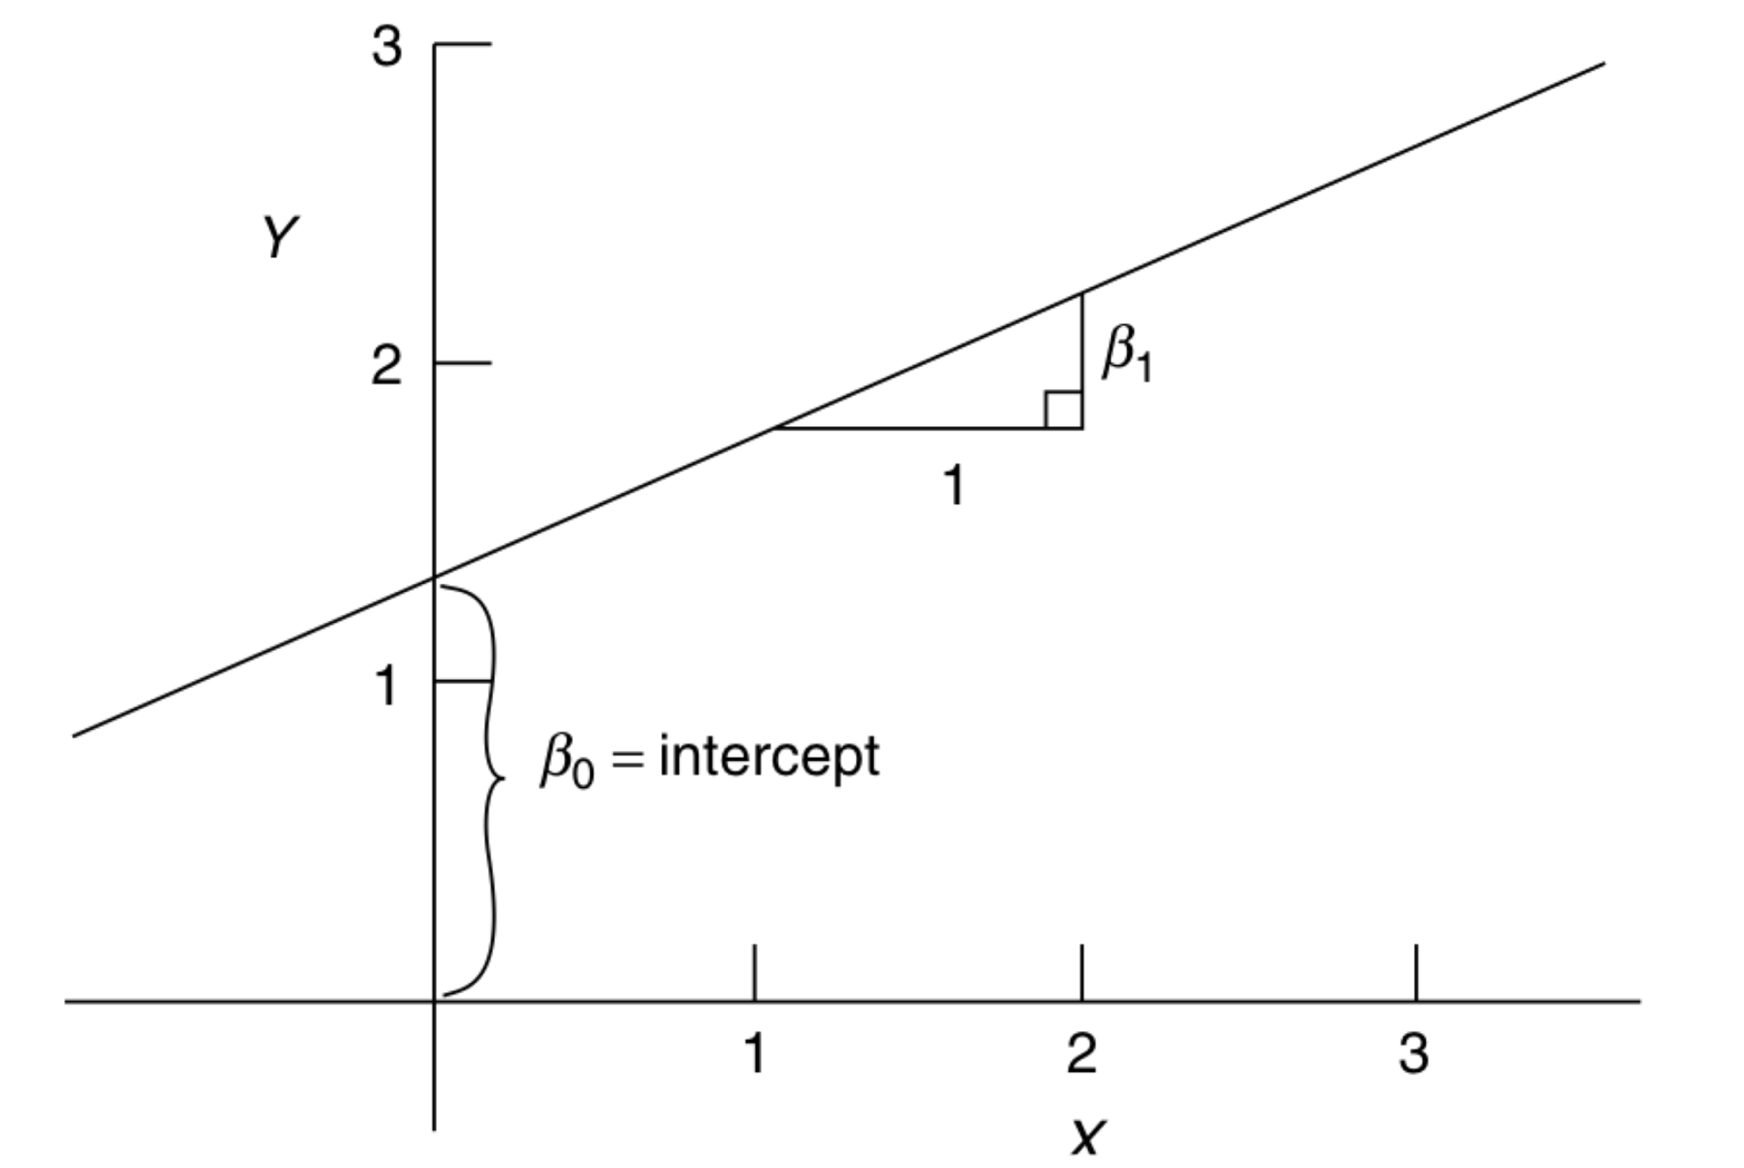
\includegraphics[width=0.8\textwidth]{fig1.png}
\end{figure}

\subsection*{Something to Notice}
Since $\sigma^2 > 0$, we have:
\[
y_i \neq E(Y|X=x_i)
\]
How to account for this difference?

We write:
\[
y_i = E(Y|X=x_i) + e_i \quad \text{(statistical error)}
\]
\textcolor{red}{where:
\[
e_i = y_i - E(Y|X=x_i)
\]
\[
\text{Note: } e_i \text{ depends on unknown parameters and is not observable.}
\]}

\subsection*{Two Important Assumptions about Errors:}
1) $E(e_i|X=x_i) = 0$ 
\textcolor{blue}{\[
\Rightarrow \text{ scatterplot (hypothetical) of } e_i \text{ vs } x_i \text{ has no patterns.}
\]}
\noindent
2) Errors are independent.
\textcolor{red}{\[
\text{Constant variance assumption implicit from above.}
\]}
\noindent
Assuming the model is true and with a sample of data $\{(X_i, Y_i); i=1, \dots, n\}$ where the pairs of $(X_i, Y_i)$ are independent.\\
\textcolor{blue}{\textbf{Q: How to estimate $\beta_0, \beta_1$?}}\\

\section*{Method of Least Squares}

\begin{figure}[H]
    \centering
    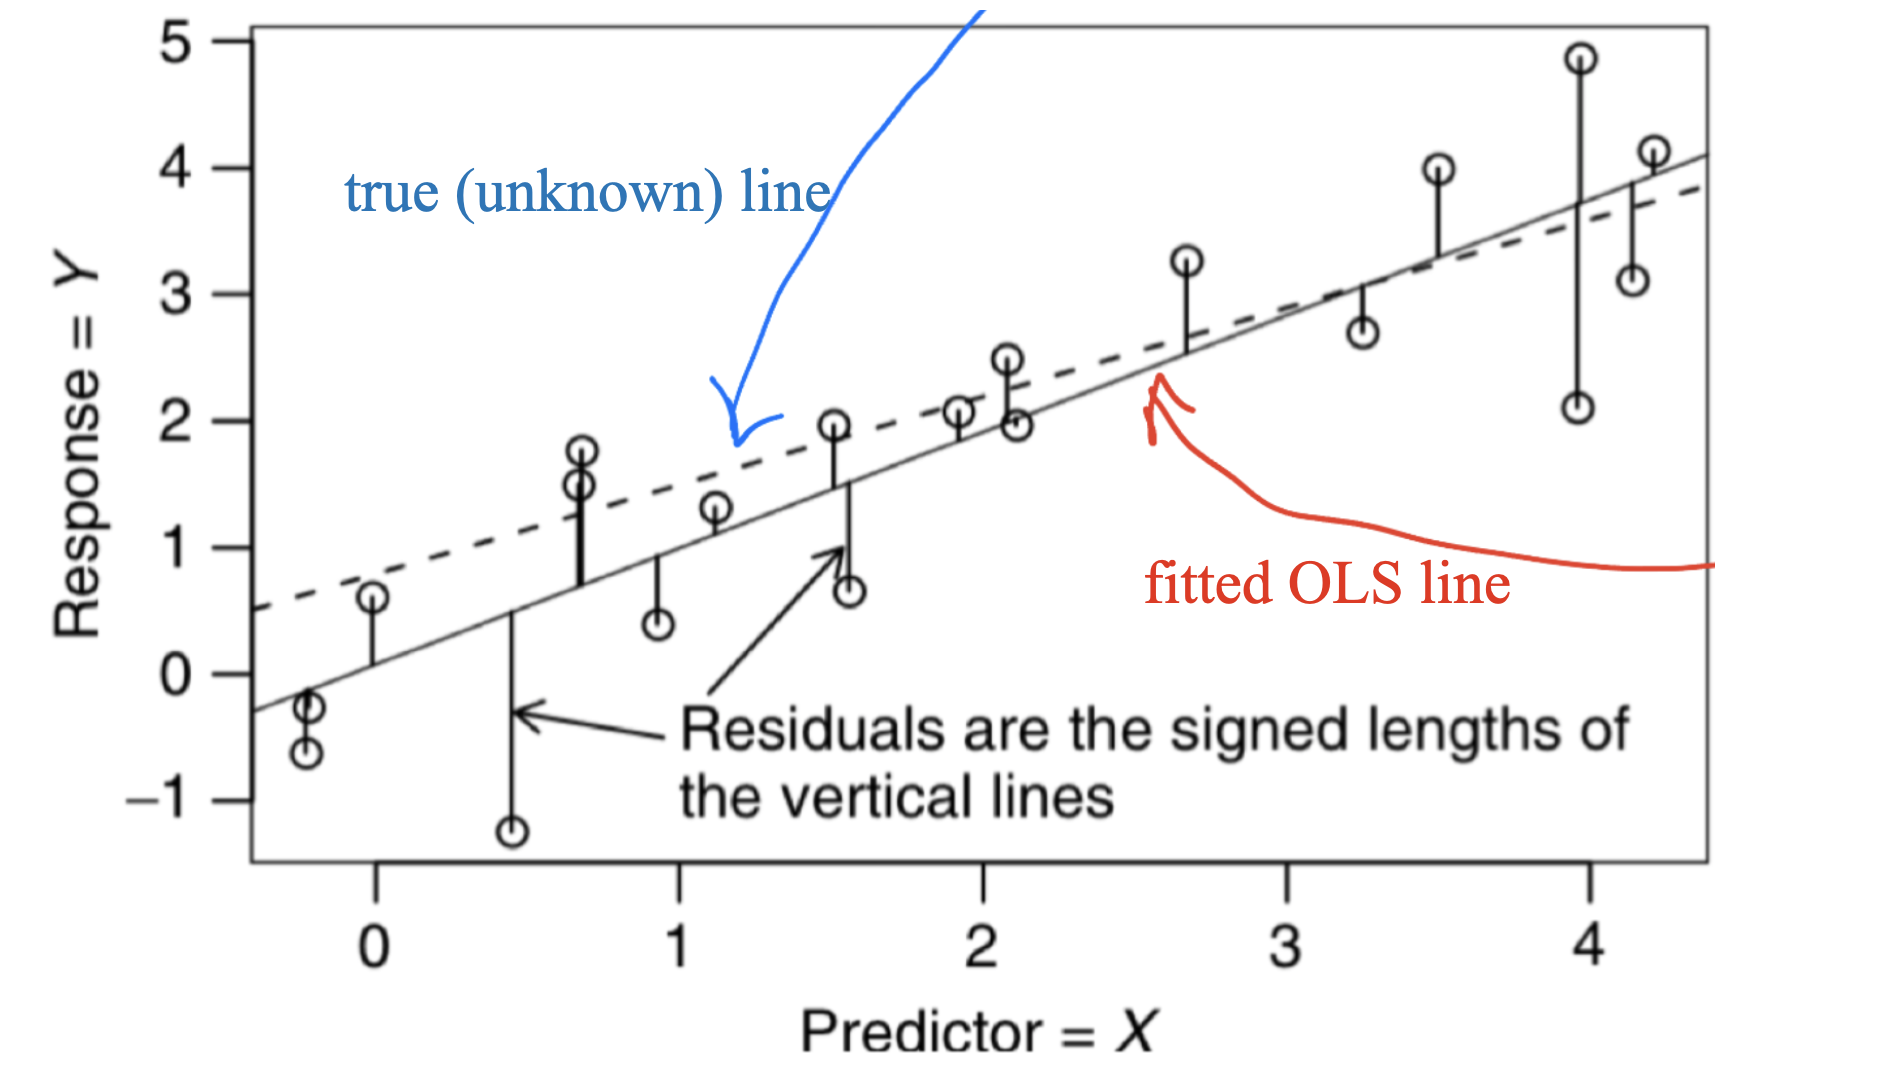
\includegraphics[width=1\textwidth]{fig2.png}
\end{figure}

\section*{Ordinary Least Squares Estimation}

The residual sum of squares (RSS) is given by:
\[
RSS(\beta_0, \beta_1) = \sum_{i=1}^{n} (y_i - \beta_0 - \beta_1 x_i)^2
\]

Taking the partial derivatives with respect to $\beta_0$ and $\beta_1$:

\[
\frac{\partial RSS(\beta_0, \beta_1)}{\partial \beta_0} = -2 \sum_{i=1}^{n} (y_i - \beta_0 - \beta_1 x_i) = 0
\]

\[
\frac{\partial RSS(\beta_0, \beta_1)}{\partial \beta_1} = -2 \sum_{i=1}^{n} x_i (y_i - \beta_0 - \beta_1 x_i) = 0
\]

From this, we derive the normal equations:
\[
\beta_0 n + \beta_1 \sum x_i = \sum y_i
\]
\[
\beta_0 \sum x_i + \beta_1 \sum x_i^2 = \sum x_i y_i
\]

These are known as the "Normal Equations."

$\Rightarrow$ We can also express:
\[
SXX = \sum_{i}(x_i - \bar{x})^2 = \sum x_i^2 - n \bar{x}^2
\]
\[
SXY = \sum_{i}(x_i - \bar{x})(y_i - \bar{y}) = \sum x_i y_i - n \bar{x} \bar{y}
\]

\begin{figure}[H]
    \centering
    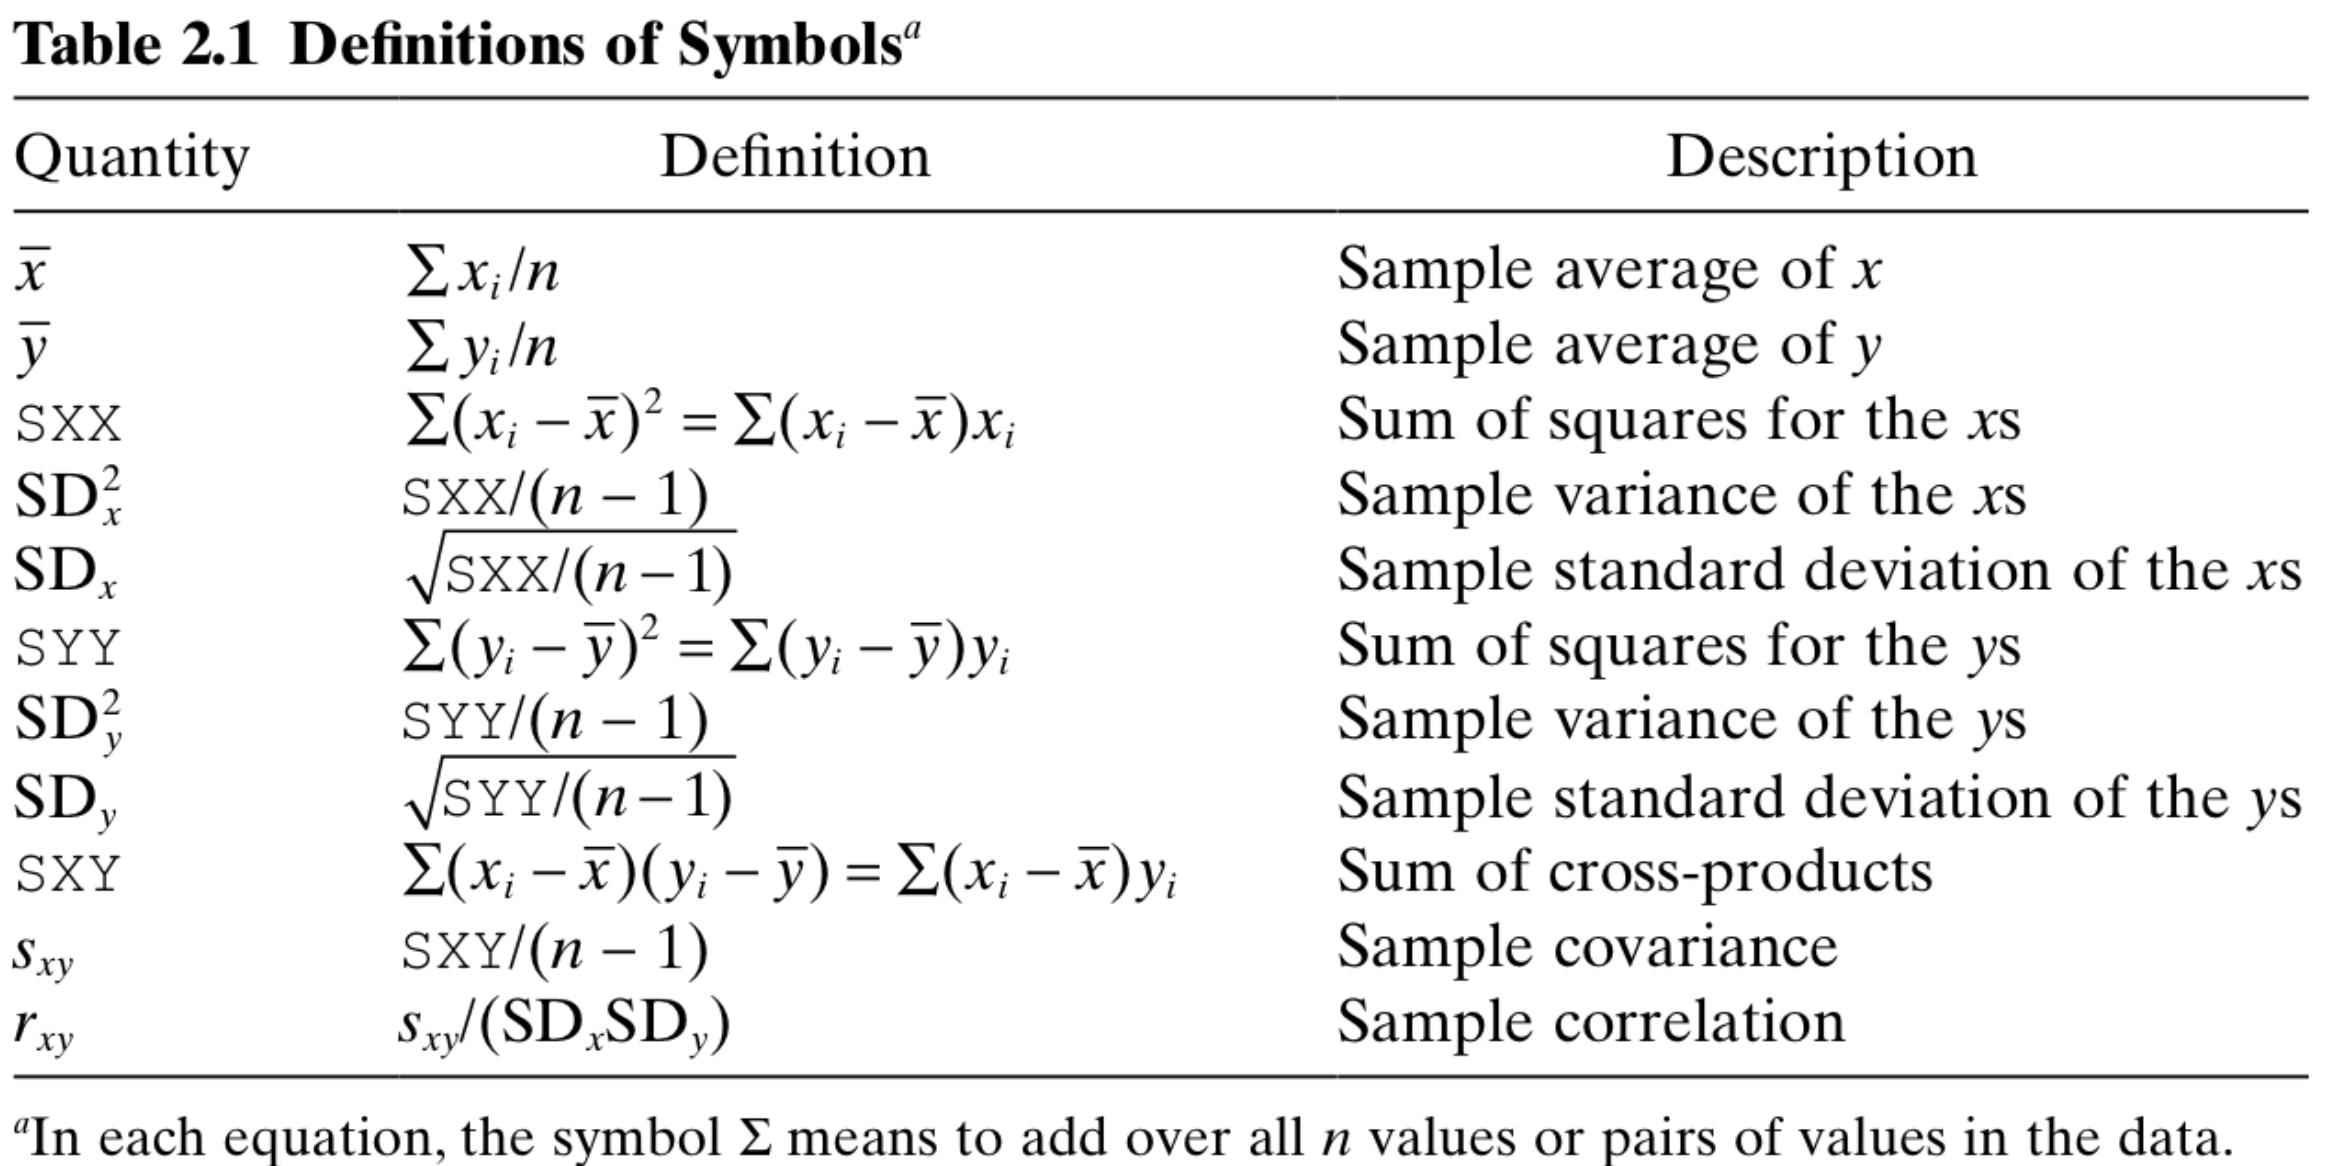
\includegraphics[width=1\textwidth]{fig3.png}
\end{figure}
\[
\Rightarrow \hat{\beta_0} = \bar{y} - \hat{\beta_1} \bar{x} \quad , \quad
\hat{\beta_1} = \frac{SXY}{SXX}
\]

\textcolor{blue}{The fitted values are:
\[
\hat{y_i} = \hat{\beta_0} + \hat{\beta_1} x_i \quad \text{for } i = 1, \dots, n
\]}

\textbf{Note:}
\[
\hat{\beta_1} = r_{xy} \frac{SD_y}{SD_x}
= r_{xy} \left( \frac{SYY}{SXX} \right)''^2
\]
\textcolor{red}{
\textbf{Note:} We are conditioning on \( X \), so by convention:
\[
\beta_0 = \beta_0|X \quad \text{and} \quad \beta_1 = \beta_1|X
\]
}
$E(\hat{\beta_1}):$

Rewrite:
\[
\hat{\beta_1} = \sum_i c_i y_i
\quad \text{ with  }
c_i = \frac{(x_i - \bar{x})}{SXX} \quad \text{(fixed)}
\]
\[
\Rightarrow E(\hat{\beta_1}) = E\left(\sum_i c_i y_i\right) = \sum_i c_i E(y_i)
= \sum_i c_i (\beta_0 + \beta_1 x_i)
= \beta_0 \sum_i c_i + \beta_1 \sum_i c_i x_i
\]
\textbf{Note:}
\[
\sum_i c_i = 0 \quad \text{and} \quad \sum_i c_i x_i = 1
\Rightarrow E(\hat{\beta_1}) = \beta_1
\]
$E(\hat{\beta_0}):$
\[
E(\hat{\beta_0}) = E(\bar{y}) - E(\hat{\beta_1}) \bar{x}
= \beta_0 + \beta_1 \bar{x} - \beta_1 \bar{x}
= \beta_0
\]
$\therefore \hat{\beta_0}$ and $\hat{\beta_1}$ are unbiased estimators of $\beta_0$ and $\beta_1$ respectively.
\[
\text{Var}(\hat{\beta_1}) = \text{Var}\left(\sum_i c_i y_i\right)
= \sum_i c_i^2 \text{Var}(y_i)
= \sigma^2 \sum_i c_i^2
= \frac{\sigma^2}{SXX}
\]
\[
\text{Var}(\hat{\beta_0}) = \text{Var}(\bar{y} - \hat{\beta_1} \bar{x})
= \text{Var}(\bar{y}) + \bar{x}^2 \text{Var}(\hat{\beta_1}) - 2 \bar{x} \, \text{Cov}(\bar{y}, \hat{\beta_1})
\]
\[
\text{Cov}(\bar{y}, \hat{\beta_1}) = \text{Cov}\left(\frac{1}{n} \sum y_i, \sum c_i y_i \right)
= \frac{1}{n} \sum c_i \, \text{Cov}(y_i, y_i)
= \frac{\sigma^2}{n} \sum c_i
= 0
\]

Since the $y_i$ are independent by assumption and $\sum c_i = 0$,
\[
\therefore \text{Var}(\hat{\beta_0}) = \sigma^2 \left( \frac{1}{n} + \frac{\bar{x}^2}{SXX} \right)
\]

\[
\text{Cov}(\hat{\beta_0}, \hat{\beta_1}) = \text{Cov}\left( \bar{y} - \hat{\beta_1} \bar{x}, \hat{\beta_1} \right)
= \text{Cov}(\bar{y}, \hat{\beta_1}) - \bar{x} \, \text{Cov}(\hat{\beta_1}, \hat{\beta_1})
\]
\[
= 0 - \sigma^2 \frac{\bar{x}}{S_{XX}}
= -\sigma^2 \frac{\bar{x}}{S_{XX}}
\]

We can use these results to get the variance of $\hat{y} = \hat{\beta_0} + \hat{\beta_1} x$ (fitted value):
\[
\text{Var}(\hat{y})\textcolor{red}{ (\text{Var}(\hat{y}|X=x)) }= \text{Var}(\hat{\beta_0} + \hat{\beta_1} x)
\]
\[
= \text{Var}(\hat{\beta_0}) + x^2 \, \text{Var}(\hat{\beta_1}) + 2x \, \text{Cov}(\hat{\beta_0}, \hat{\beta_1})
\]
\[
= \sigma^2 \left( \frac{1}{n} + \frac{\bar{x}^2}{SXX} \right) + \sigma^2 \frac{x^2}{SXX} - 2 \sigma^2 \frac{x \bar{x}}{SXX}
\]
\[
= \sigma^2 \left( \frac{1}{n} + \frac{(x - \bar{x})^2}{SXX} \right)
\]
\textcolor{blue}{\textbf{Interesting Fact:}
\[
\hat{E}(Y | X = \bar{x}) = \bar{y} - \hat{\beta_1} \bar{x} = \bar{y}
\]
$\therefore$ the fitted line passes through the point $(\bar{x}, \bar{y})$.
}
\begin{figure}[H]
    \centering
    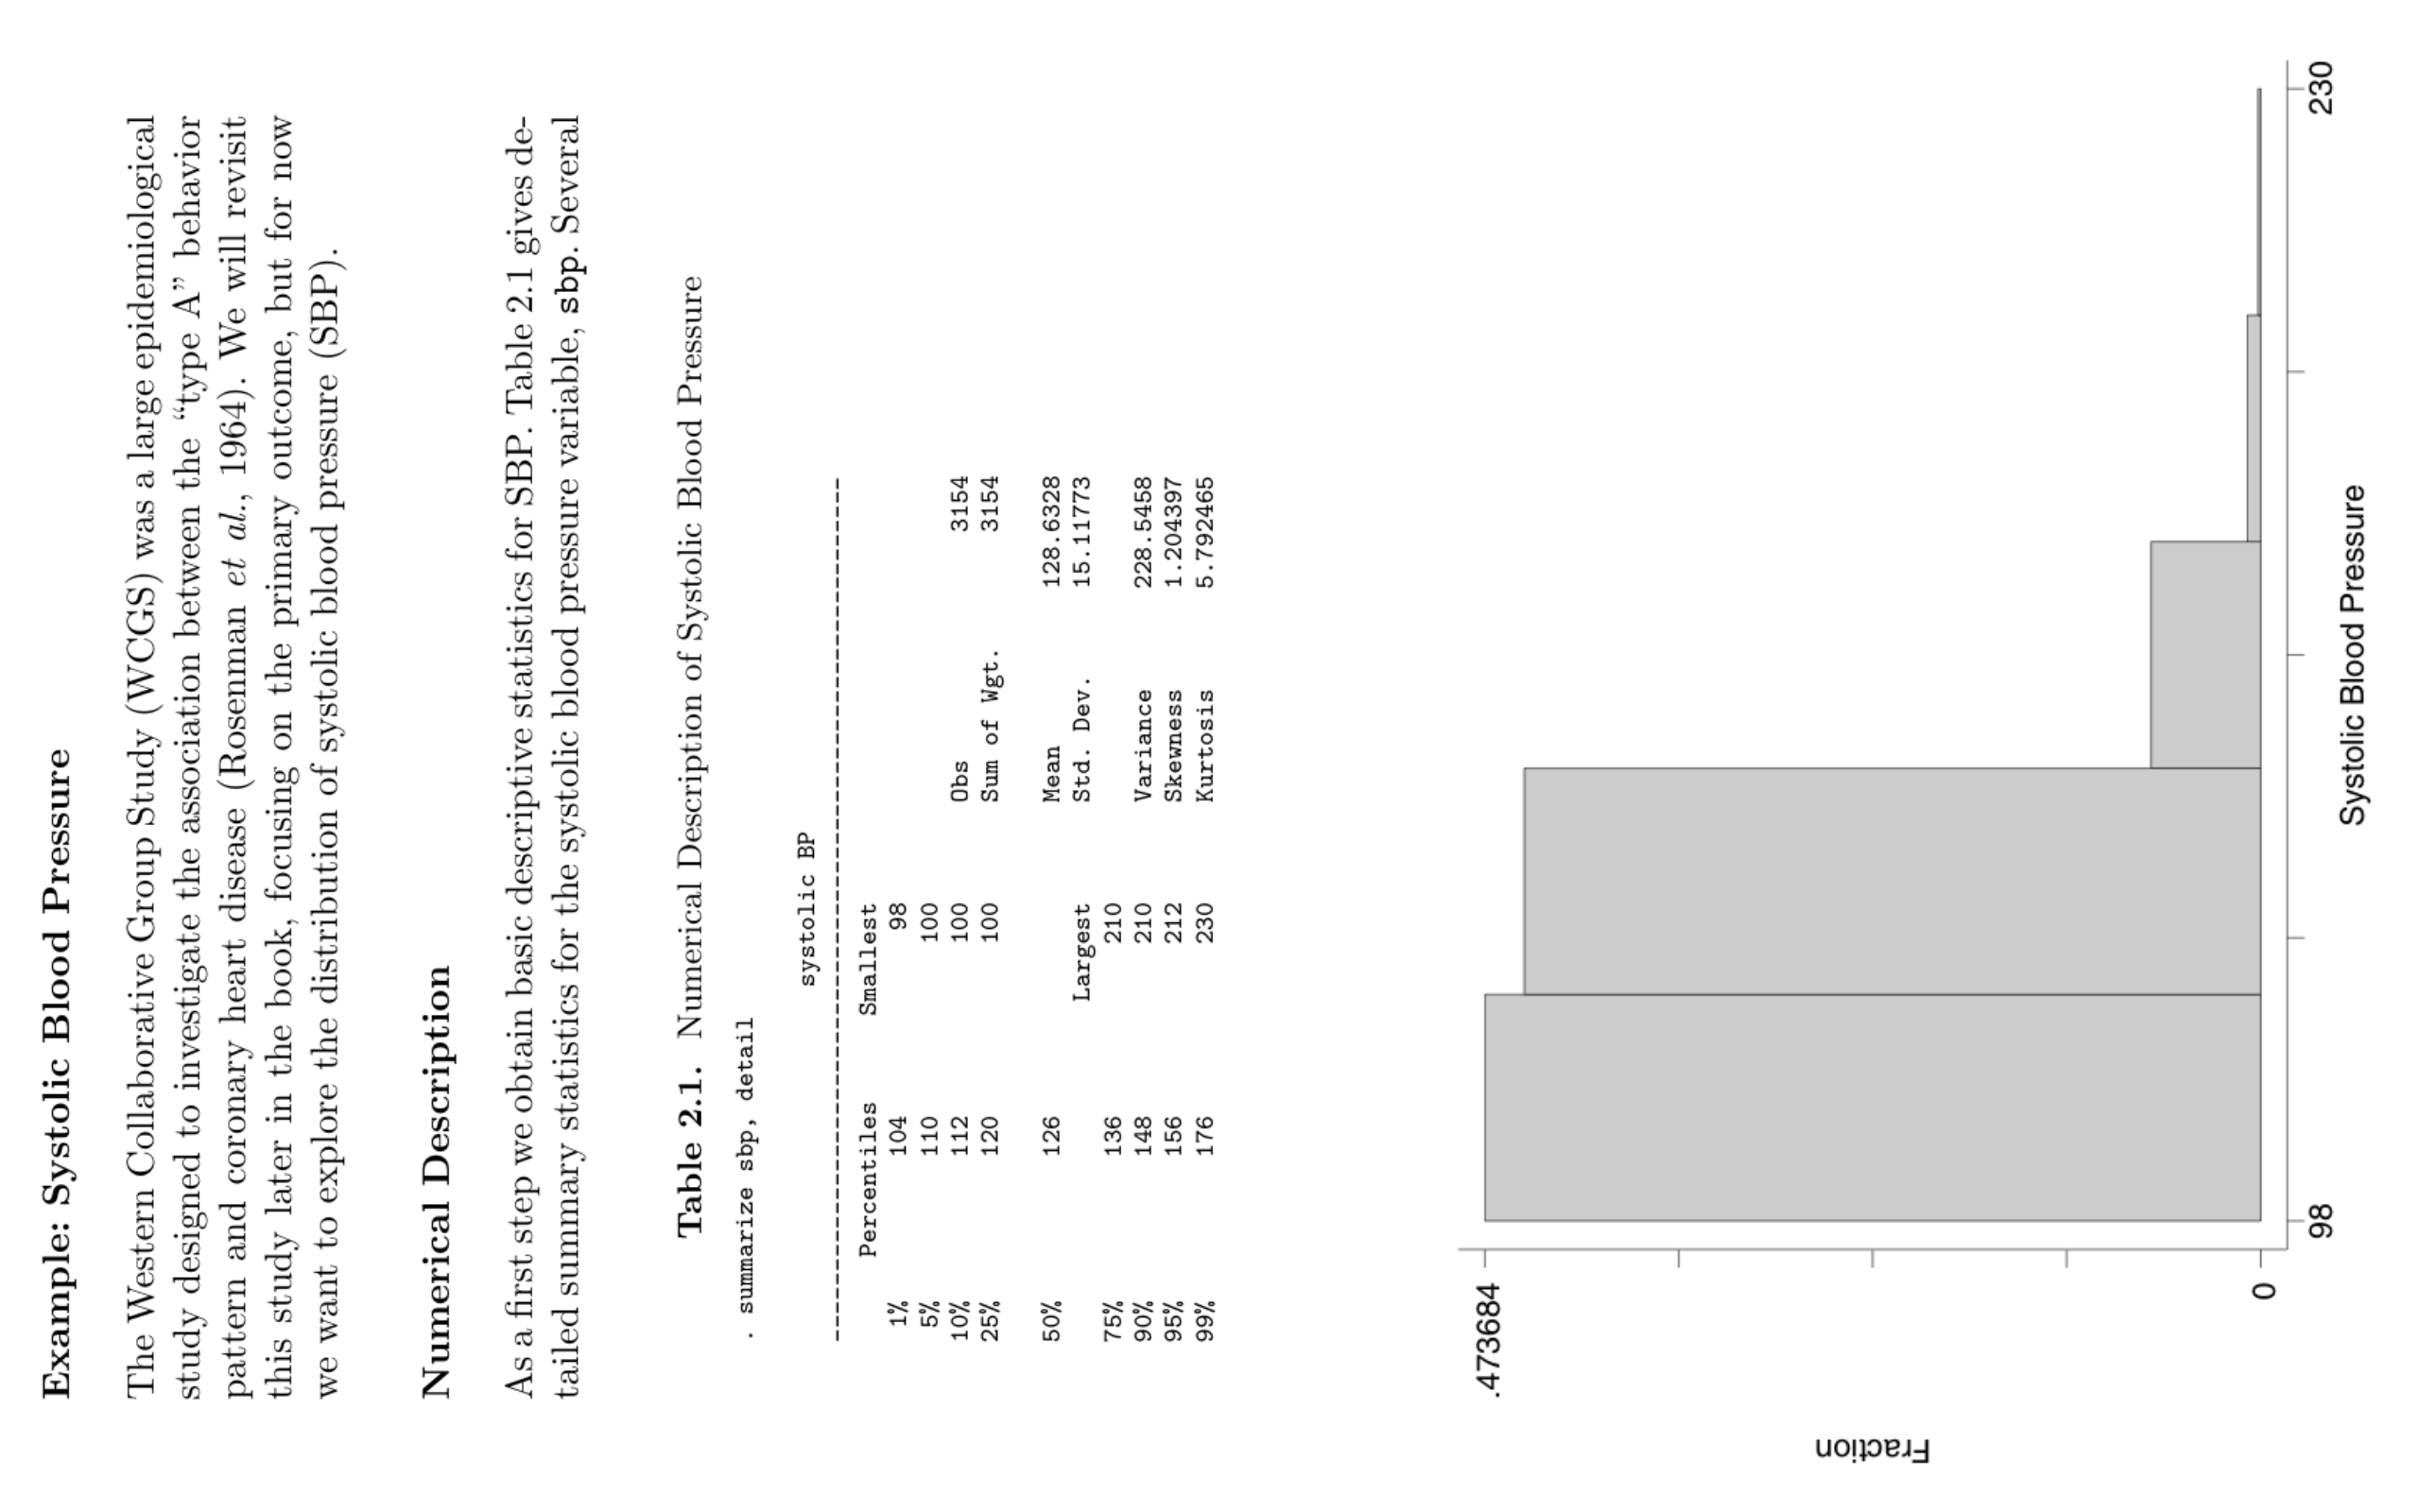
\includegraphics[height=0.65\textheight, angle=270]{fig4.png}
\end{figure}

\begin{figure}[H]
    \centering
    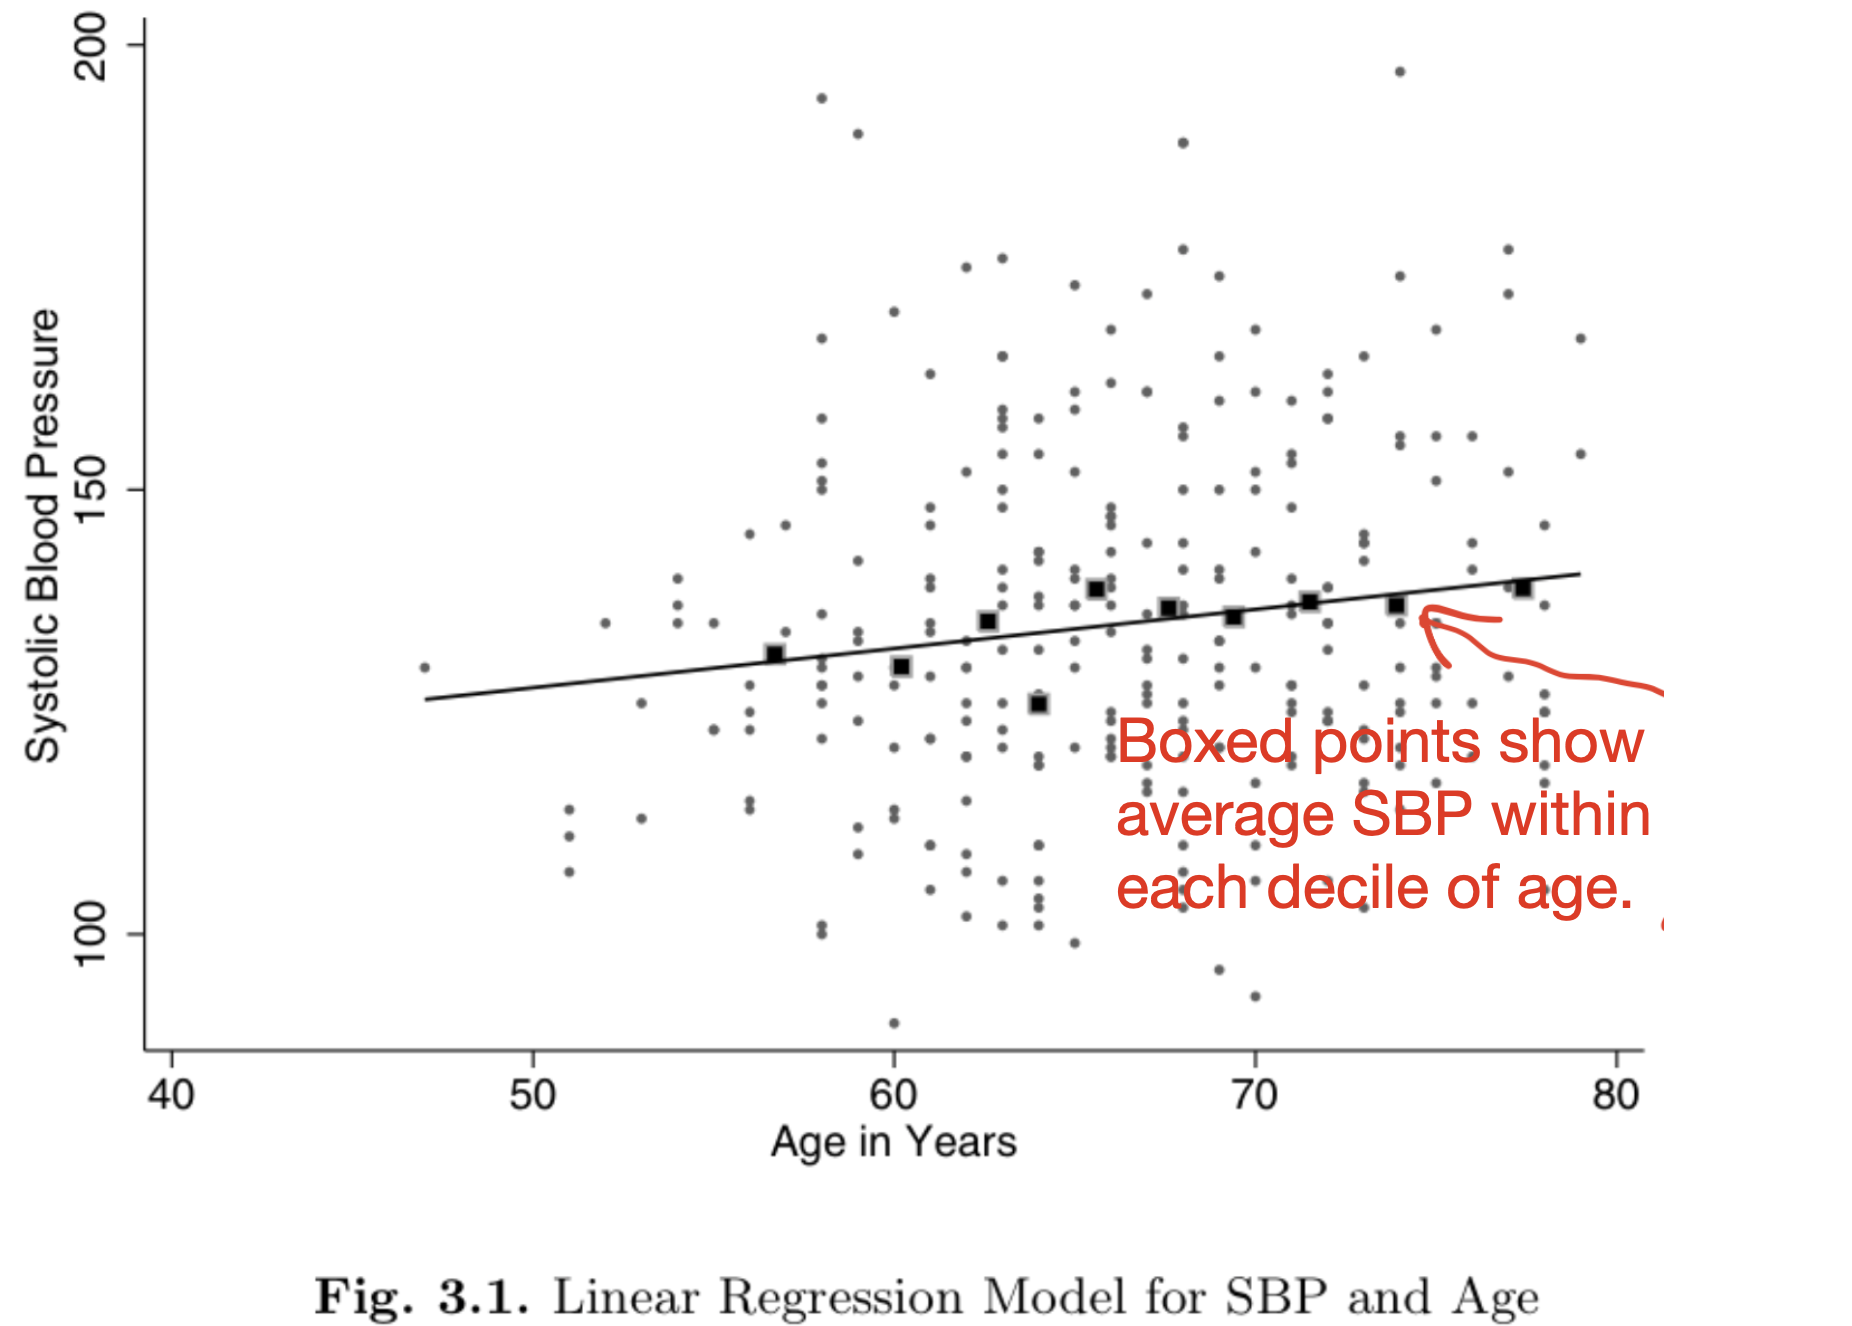
\includegraphics[width=1\textwidth]{fig5.png}
\end{figure}
\noindent
Here:\\
$
\hat{\beta_0} = 105.7 \quad \Rightarrow \quad \text{average SBP at age = 0 (not meaningful here)}
$\\
$
\hat{\beta_1} = 0.44 \quad \Rightarrow \quad$ among women with heart disease, average SBP increases by 0.44 mmHg for each 1 year increase in age

\section*{Estimating the Variance $\sigma^2$}

\textcolor{blue}{Logic: $\sigma^2$ is essentially the average squared size of the $e_i^2$. 
\[
\Rightarrow \hat{\sigma}^2 \text{ is obtained by averaging squared residuals}.
\]
}
Under the assumption that errors are uncorrelated random variables with mean 0 and variance $\sigma^2$, we have:
\[
\Rightarrow \frac{RSS}{n} = \sum_{i} \frac{\hat{e}_i^2}{n} = \hat{\sigma}^2
\quad 
\textcolor{red}{\text{(Candidate to estimate } \sigma^2\text{)}.}
\]
But:
\[
E({\overset{\sim}{\sigma}}^2) \neq \sigma^2 \quad \text{(biased)}.
\]
We must use instead:\textcolor{blue}{$\quad n-2 : $\text{\# parameters estimated (df)}}.
\[
\hat{\sigma}^2 = \frac{RSS}{n-2}\quad
\]
\[
\text{Now: }E(\hat{\sigma}^2) = \sigma^2.
\]

\section*{Confidence Intervals and t-Tests}
\begin{figure}[H]
    \centering
    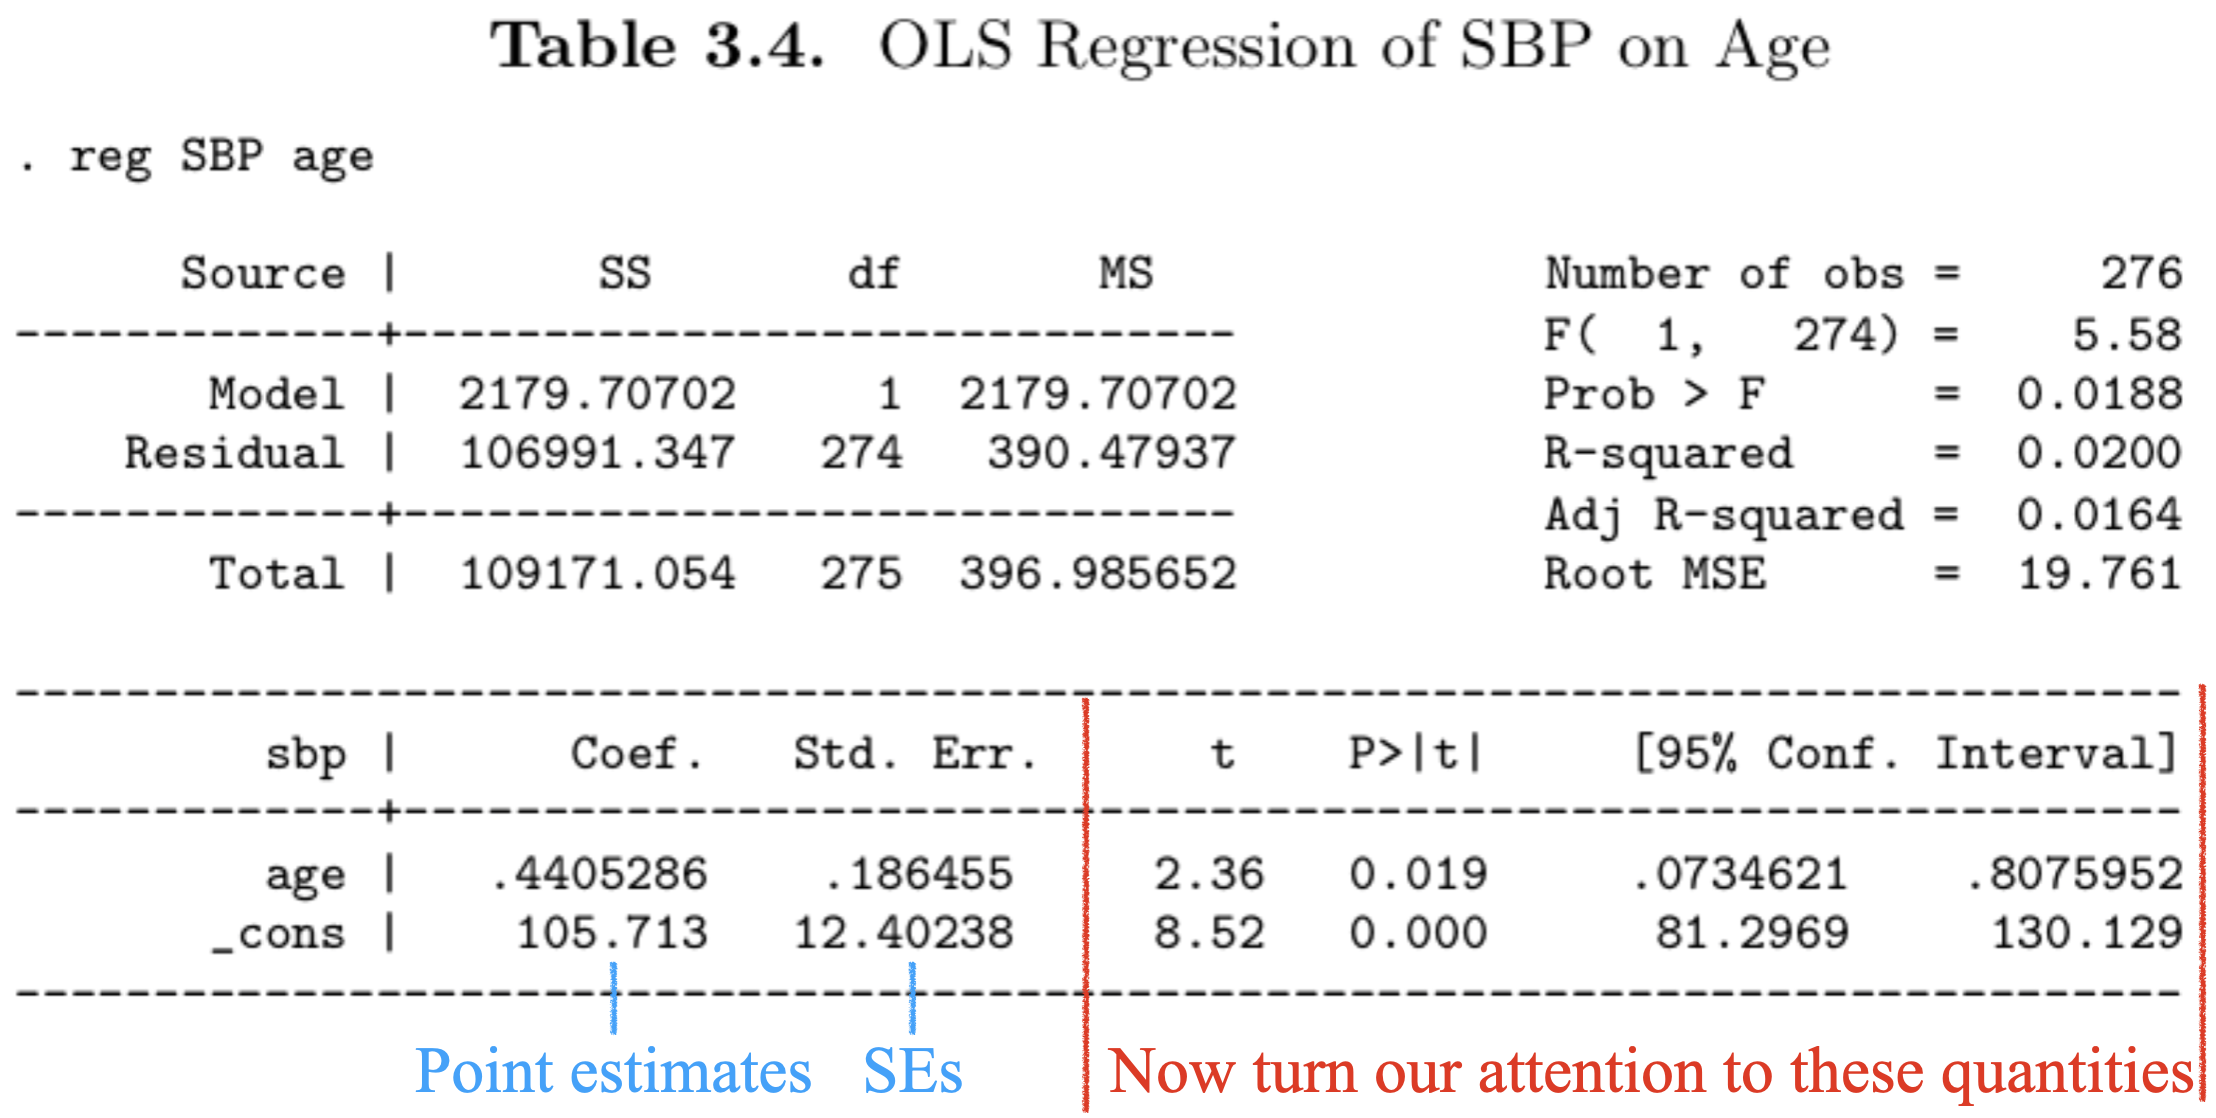
\includegraphics[width=1\textwidth]{fig6.png}
\end{figure}

\noindent
Confidence intervals result in interval estimates for true parameters. \\
Tests provide a methodology to make decisions concerning the value of a parameter or fitted value.

\noindent
When errors are assumed to also be normally distributed:\\
$\Rightarrow$ Parameter estimates and fitted values will be normally distributed.\\
$\Rightarrow$ All linear combinations of the $ y_i $ and hence the $ e_i $ .\\
Confidence intervals (CIs) and tests are based on t-distribution theory:\\
 - Appropriate with normal estimates but using $\hat{\sigma}^2$ to estimate $ \sigma^2$.\\
 - t-distribution is indexed by degrees of freedom (df) associated with $\hat{\sigma}^2$:
\[
\Rightarrow t(\alpha/2, cl)
\]
\textcolor{red}{Quantile for $ \alpha / 2 \times 100\% $ in upper tail of the t-distribution, cl $\rightarrow$ df} \\
\textbf{The intercept}
First note:
\[
SE(\hat{\beta_0}) = \sqrt{\text{Var}(\hat{\beta_0})}
= \hat{\sigma} \left( \frac{1}{n} + \frac{\bar{x}^2}{SXX} \right) \quad \textcolor{red}{\text{(plugging in } \hat{\sigma} \text{ for } \sigma \text{)}}
\]
The $(1-\alpha) \times 100\%$ confidence interval (CI) for $\beta_0$ is:
\[
\hat{\beta_0} - t\left(\alpha/2, n-2\right) SE(\hat{\beta_0}) \leq \beta_0 \leq \hat{\beta_0} + t\left(\alpha/2, n-2\right) SE(\hat{\beta_0})
\]
\begin{figure}[H]
    \centering
    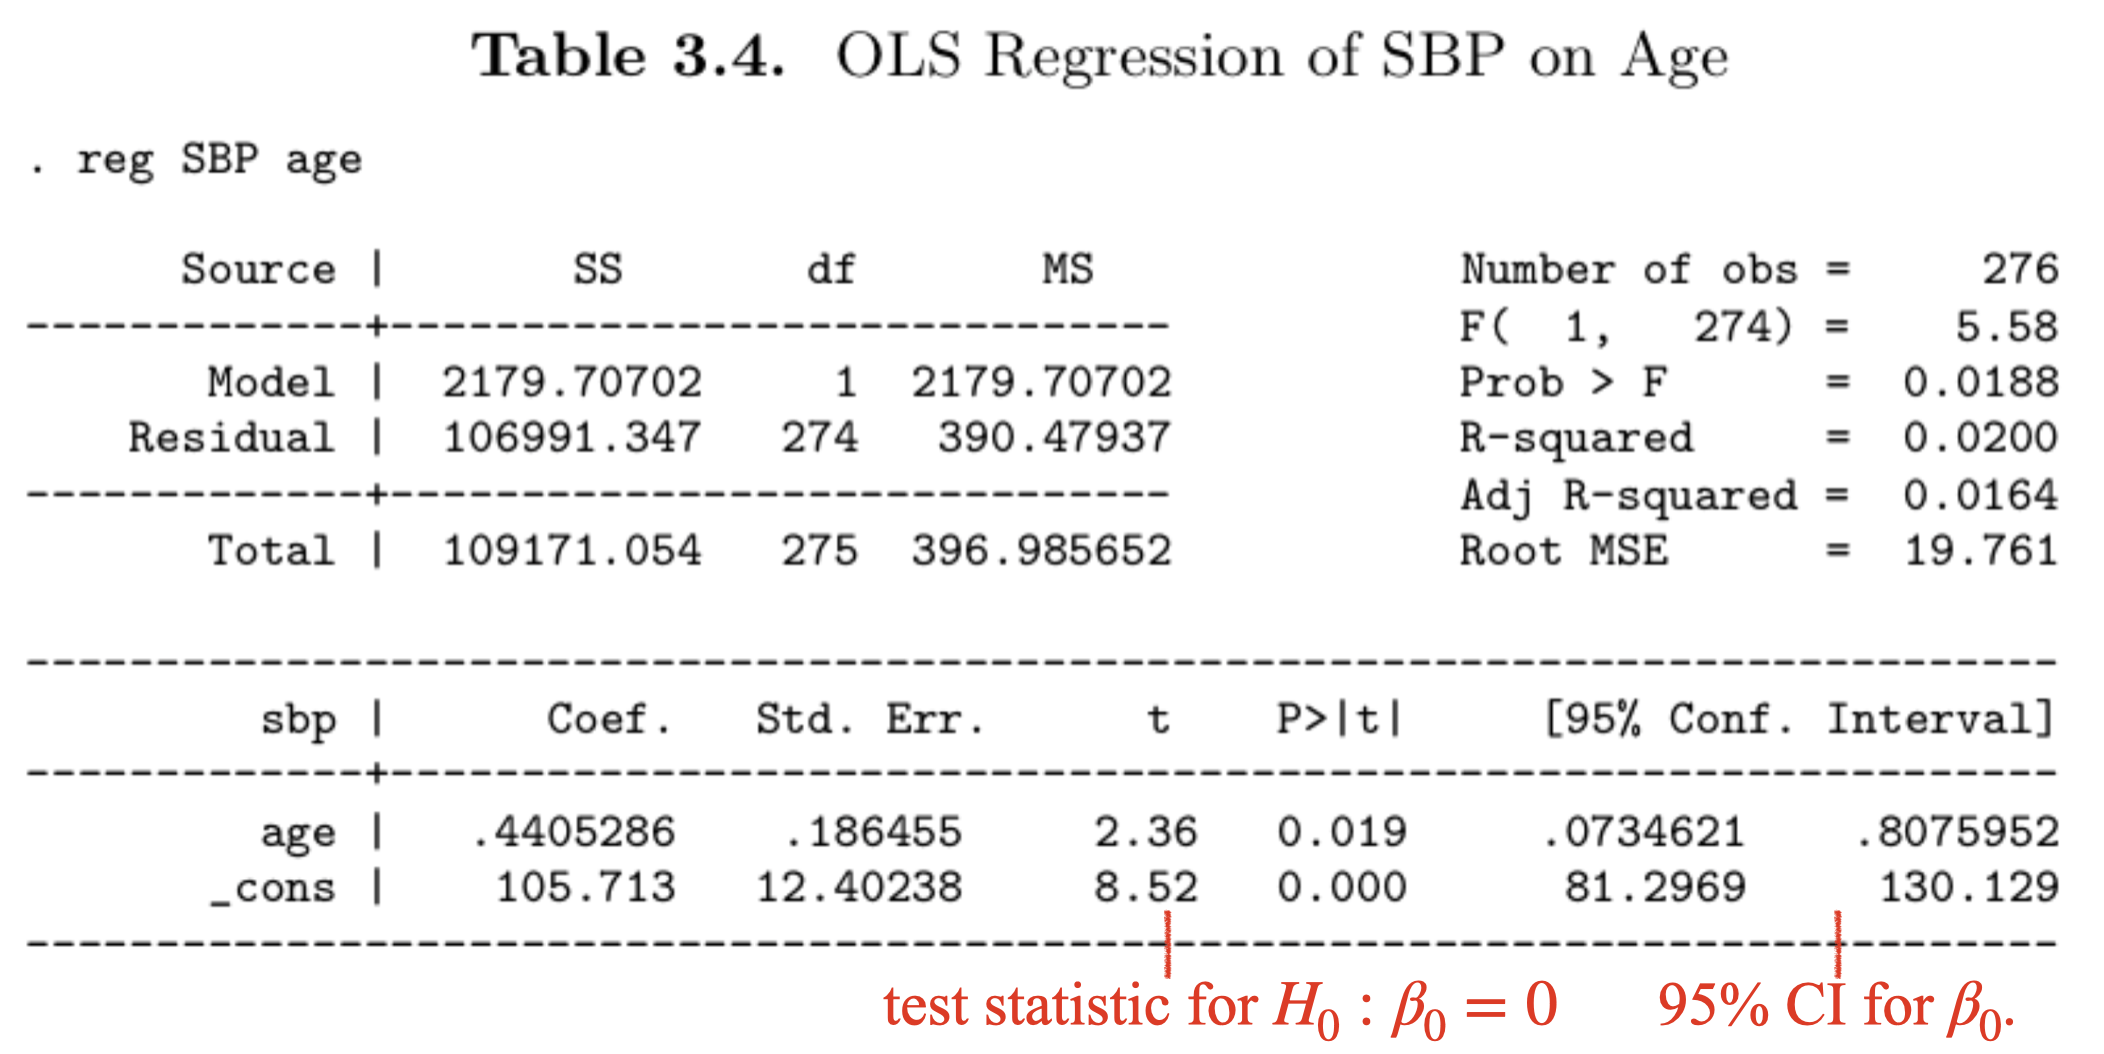
\includegraphics[width=1\textwidth]{fig7.png}
\end{figure}
\noindent
\textbf{A hypothesis test of: }\textcolor{red}{\text{(often interested in } $\beta_0^* = 0 $\text{)}}
\[
H_0: \beta_0 = \beta_0^* , 
H_1: \beta_0 \neq \beta_0^* \quad 
\]
The test statistic is:
\[
t = \frac{\beta_0 - \beta_0^*}{SE(\hat{\beta_0})} \quad \overset{H_0}{\sim} \quad t(n-2)
\]
\[
\Rightarrow p\text{-value} \quad (\approx 0 \text{ in above Table 3.4}).
\]
\textcolor{blue}{Note: Since $H_1$ is two-sided, the p-value corresponds to $P\left(t(n-2) > |t|\right)$.}
\subsection*{The Slope}

A $(1-\alpha) \times 100\%$ confidence interval (CI) for the slope is the set of $\beta_1$ such that:
$\hat{\beta_1} - t\left(\alpha/2, n-2\right) SE(\hat{\beta_1}) \leq \beta_1 \leq \hat{\beta_1} + t\left(\alpha/2, n-2\right) SE(\hat{\beta_1})$
\[
\left[\text{recall } SE(\hat{\beta_1}) = \frac{\hat{\sigma}}{\sqrt{SXX}} = \sqrt{\text{Var}(\hat{\beta_1})}\right]
\]
\begin{figure}[H]
    \centering
    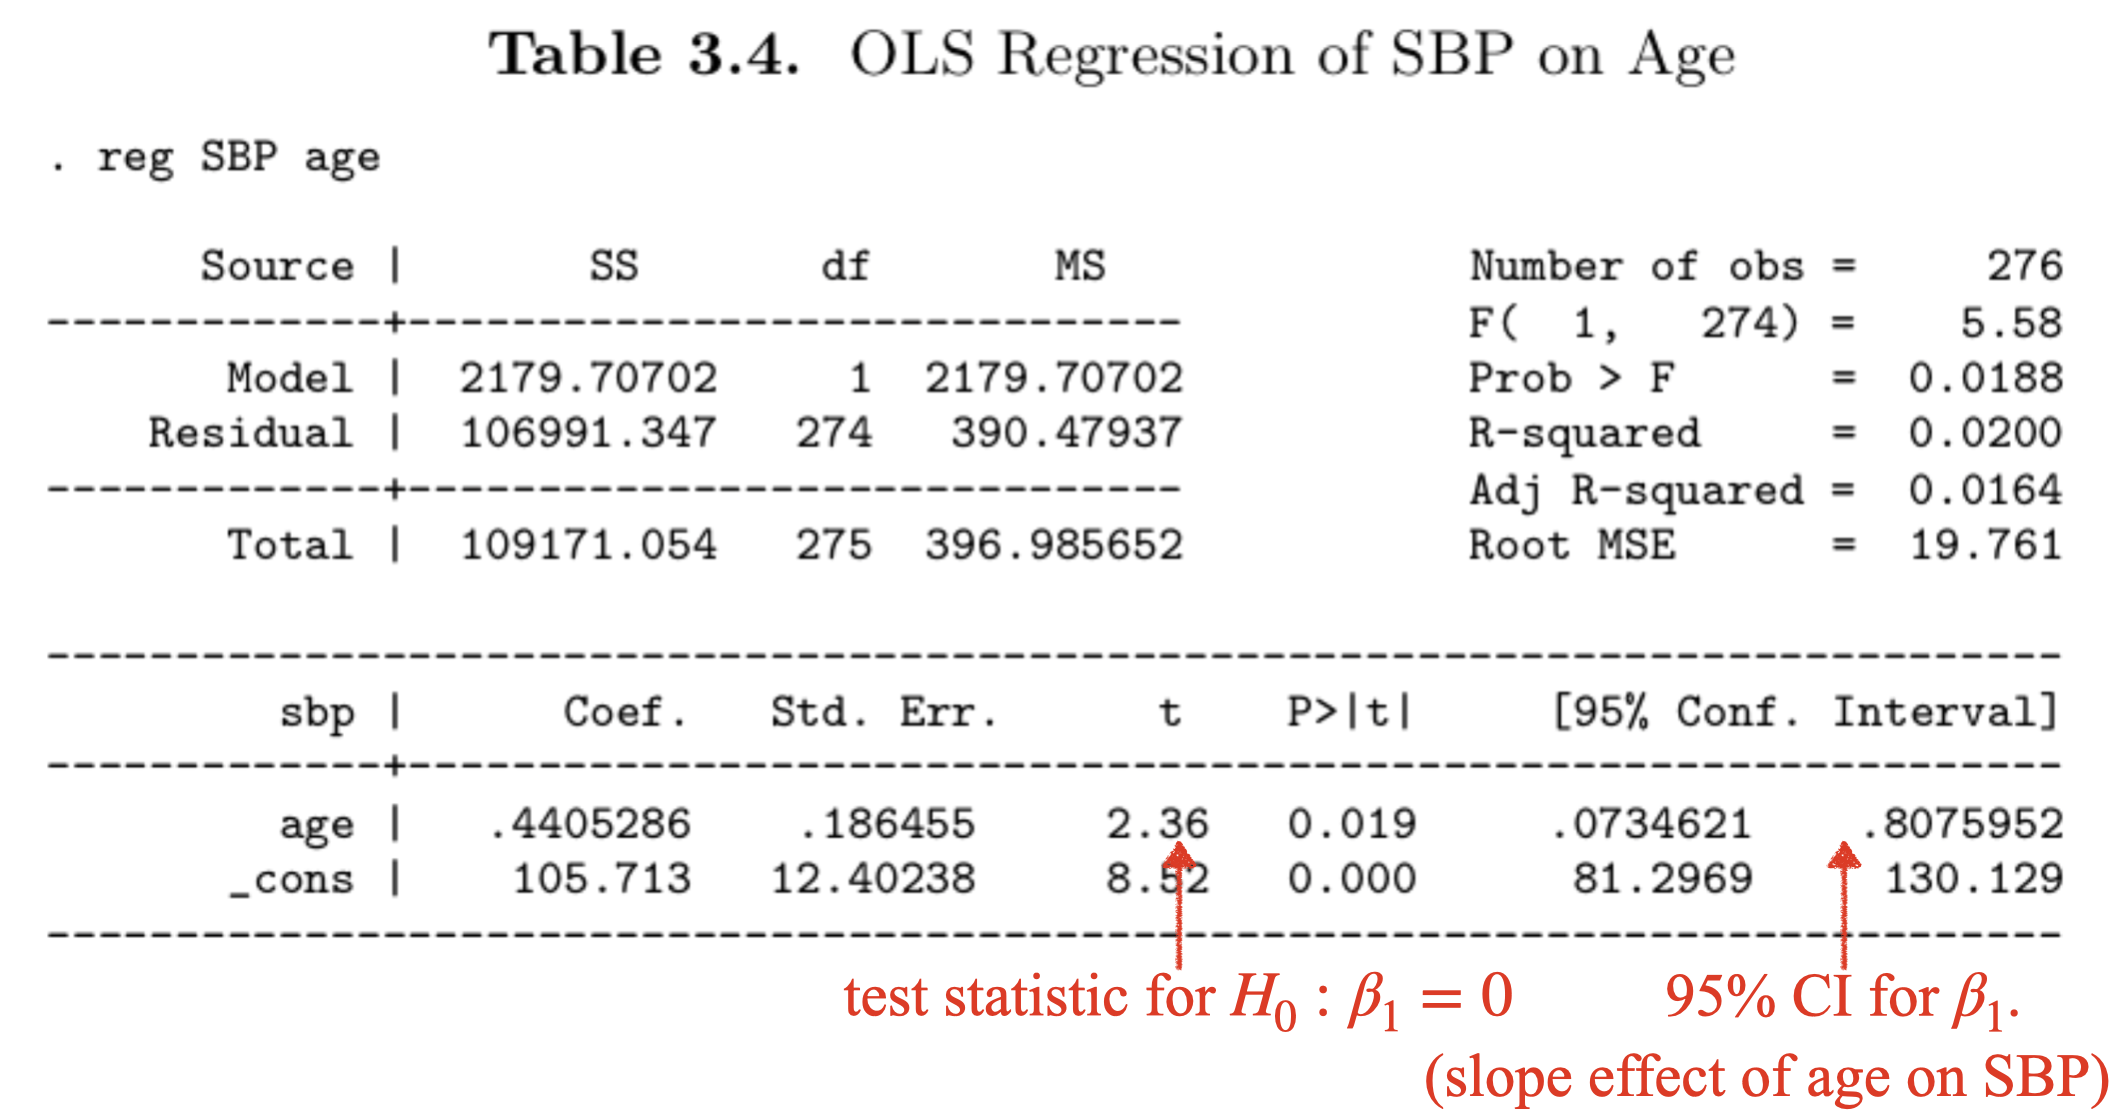
\includegraphics[width=1\textwidth]{fig8.png}
\end{figure}
\noindent
\textbf{A Hypothesis Test of Particular Interest}\\
A hypothesis test of:
\[
H_0: \beta_1 = 0, 
H_1: \beta_1 \neq 0
\]
Similar to testing the intercept, the test statistic is:
\[
t = \frac{\hat{\beta_1} - 0}{SE(\hat{\beta_1})} \quad \overset{H_0}{\sim} \quad t(n-2)
\]
The p-value (two-sided) is:
\[
P\left( t(n-2) > |t| \right)
\]
\textcolor{blue}{In above Table 3.4, p = 0.019, suggesting that SBP is linearly related to age.}

\section*{Prediction}
\noindent
Estimated mean function $\hat{E}(Y|X)$ can be used to obtain values of response for given values of $X$.\\
Two important classes:
\begin{enumerate}
    \item \textbf{Prediction} – new case $(X^*)$ that was not used to estimate parameters.
    \item \textbf{Fitted values} – want to estimate $E(Y|X = x^*)$.
\end{enumerate}
Let's focus on prediction first. That is, we want to estimate $Y^*$ at a value $x^*$ (not yet observed).\\
Must assume the data used to estimate $E(Y|X)$ is relevant to the new case.\\
Given this, a point prediction of $y^*$ is:
\[
\hat{y^*} = \hat{\beta_0} + \hat{\beta_1} x^*
\]
\textcolor{blue}{This is a prediction of yet unobserved $y^*$.}

\noindent
\textcolor{red}{Assuming the model is correct: $y^* = \beta_0 + \beta_1 x^* + e^* $}\\
\textcolor{blue}{$e^* : $ New random error with same assumptions.}\\
\textcolor{blue}{Note: Even if $\beta_0, \beta_1$ were known, predictions would not match true values perfectly. They would be off by a random quantity with variance $\sigma^2$.}

\noindent
Two sources of variation:
\begin{enumerate}
    \item Uncertainty in $\hat{\beta_0}, \hat{\beta_1}$ \textcolor{red}{$\Rightarrow \text{var}(\hat{y})$}
    \item Variance of $e^*$
\end{enumerate}
Combining these:
\[
\text{Var}(\tilde{y}^* | X = x^*) = \sigma^2 \left( \frac{1}{n} + \frac{(x^* - \bar{x})^2}{SXX} \right) + \sigma^2
\]
\textcolor{red}{\quad \quad \quad \quad \quad \quad \quad \quad \quad \quad \quad \quad This is the variance of $\hat{y} \uparrow$}
\[
\therefore SE(\tilde{y}^* | X = x^*) = \sqrt{\text{Var}(\tilde{y}^* | X = x^*)}
\]
We can define a $(1-\alpha) \times 100\%$ prediction interval for $y^*$ (true value) as:
\[
\tilde{y}^* \pm t\left(\alpha/2 n-2\right) SE(\tilde{y}^*)
\]
\[
\textcolor{red}{\tilde{y}^* \equiv \hat{E}(Y | X = x^*)} \quad \textcolor{red}{SE(\tilde{y}^*) \equiv SE(\tilde{y}^*| X = x^*)}
\]
Using previous notation:
\[
\tilde{y}^* - t\left(\alpha/2, n-2\right) SE(\tilde{y}^*) \leq y^* \leq \tilde{y}^* + t\left(\alpha/2, n-2\right) SE(\tilde{y}^*)
\]
Now move to the fitted values. Here, we want to estimate:
\[
E(Y | X = x^*)
\]
Point estimate:
\[
\hat{y} = \hat{\beta_0} + \hat{\beta_1} x^* = \hat{E}(Y | X = x^*)
\]
Standard error of the fitted value:
\[
SE(\hat{y} | X = x^*) = \hat{\sigma} \left( \frac{1}{n} + \frac{(x^* - \bar{x})^2}{SXX} \right)''^{2}
\]
\[
\quad \quad \quad \quad \quad \textcolor{red}{\sqrt{\text{Var}(\hat{y} | X = x^*)} \uparrow}
\]

A $(1-\alpha) \times 100\%$ CI for $E(Y | X = x^*)$ is:
\[
\hat{y} - t\left(\alpha/2, n-2\right) SE(\hat{y}) \leq E(Y | X = x^*) \leq \hat{y} + t\left(\alpha/2, n-2\right) SE(\hat{y})
\]
\[
\textcolor{red}{\hat{y}^* \equiv \hat{E}(Y | X = x^*)} \quad \textcolor{red}{SE(\hat{y}^*) \equiv SE(\hat{y}^*| X = x^*)}
\]

\section*{Coefficient of Determination, $R^2$}
\noindent
Ignoring the predictor, the best prediction of $y$ is $\bar{y}$.\\
The total sum of squares (SYY) represents the observed total variation, ignoring all predictors:
\[
SYY = \sum_i (y_i - \bar{y})^2
\]
The sum of squares due to regression (SS$_{\text{reg}}$) is:
\[
SS_{\text{reg}} = SYY - RSS
\]
\[
= SYY - \left(SYY - \frac{(SXY)^2}{SXX}\right)
\]
\[
= \frac{(SXY)^2}{SXX}
\]
\[
\Rightarrow \frac{SS_{\text{reg}}}{SYY} = 1 - \frac{RSS}{SYY}
\]
\begin{figure}[H]
    \centering
    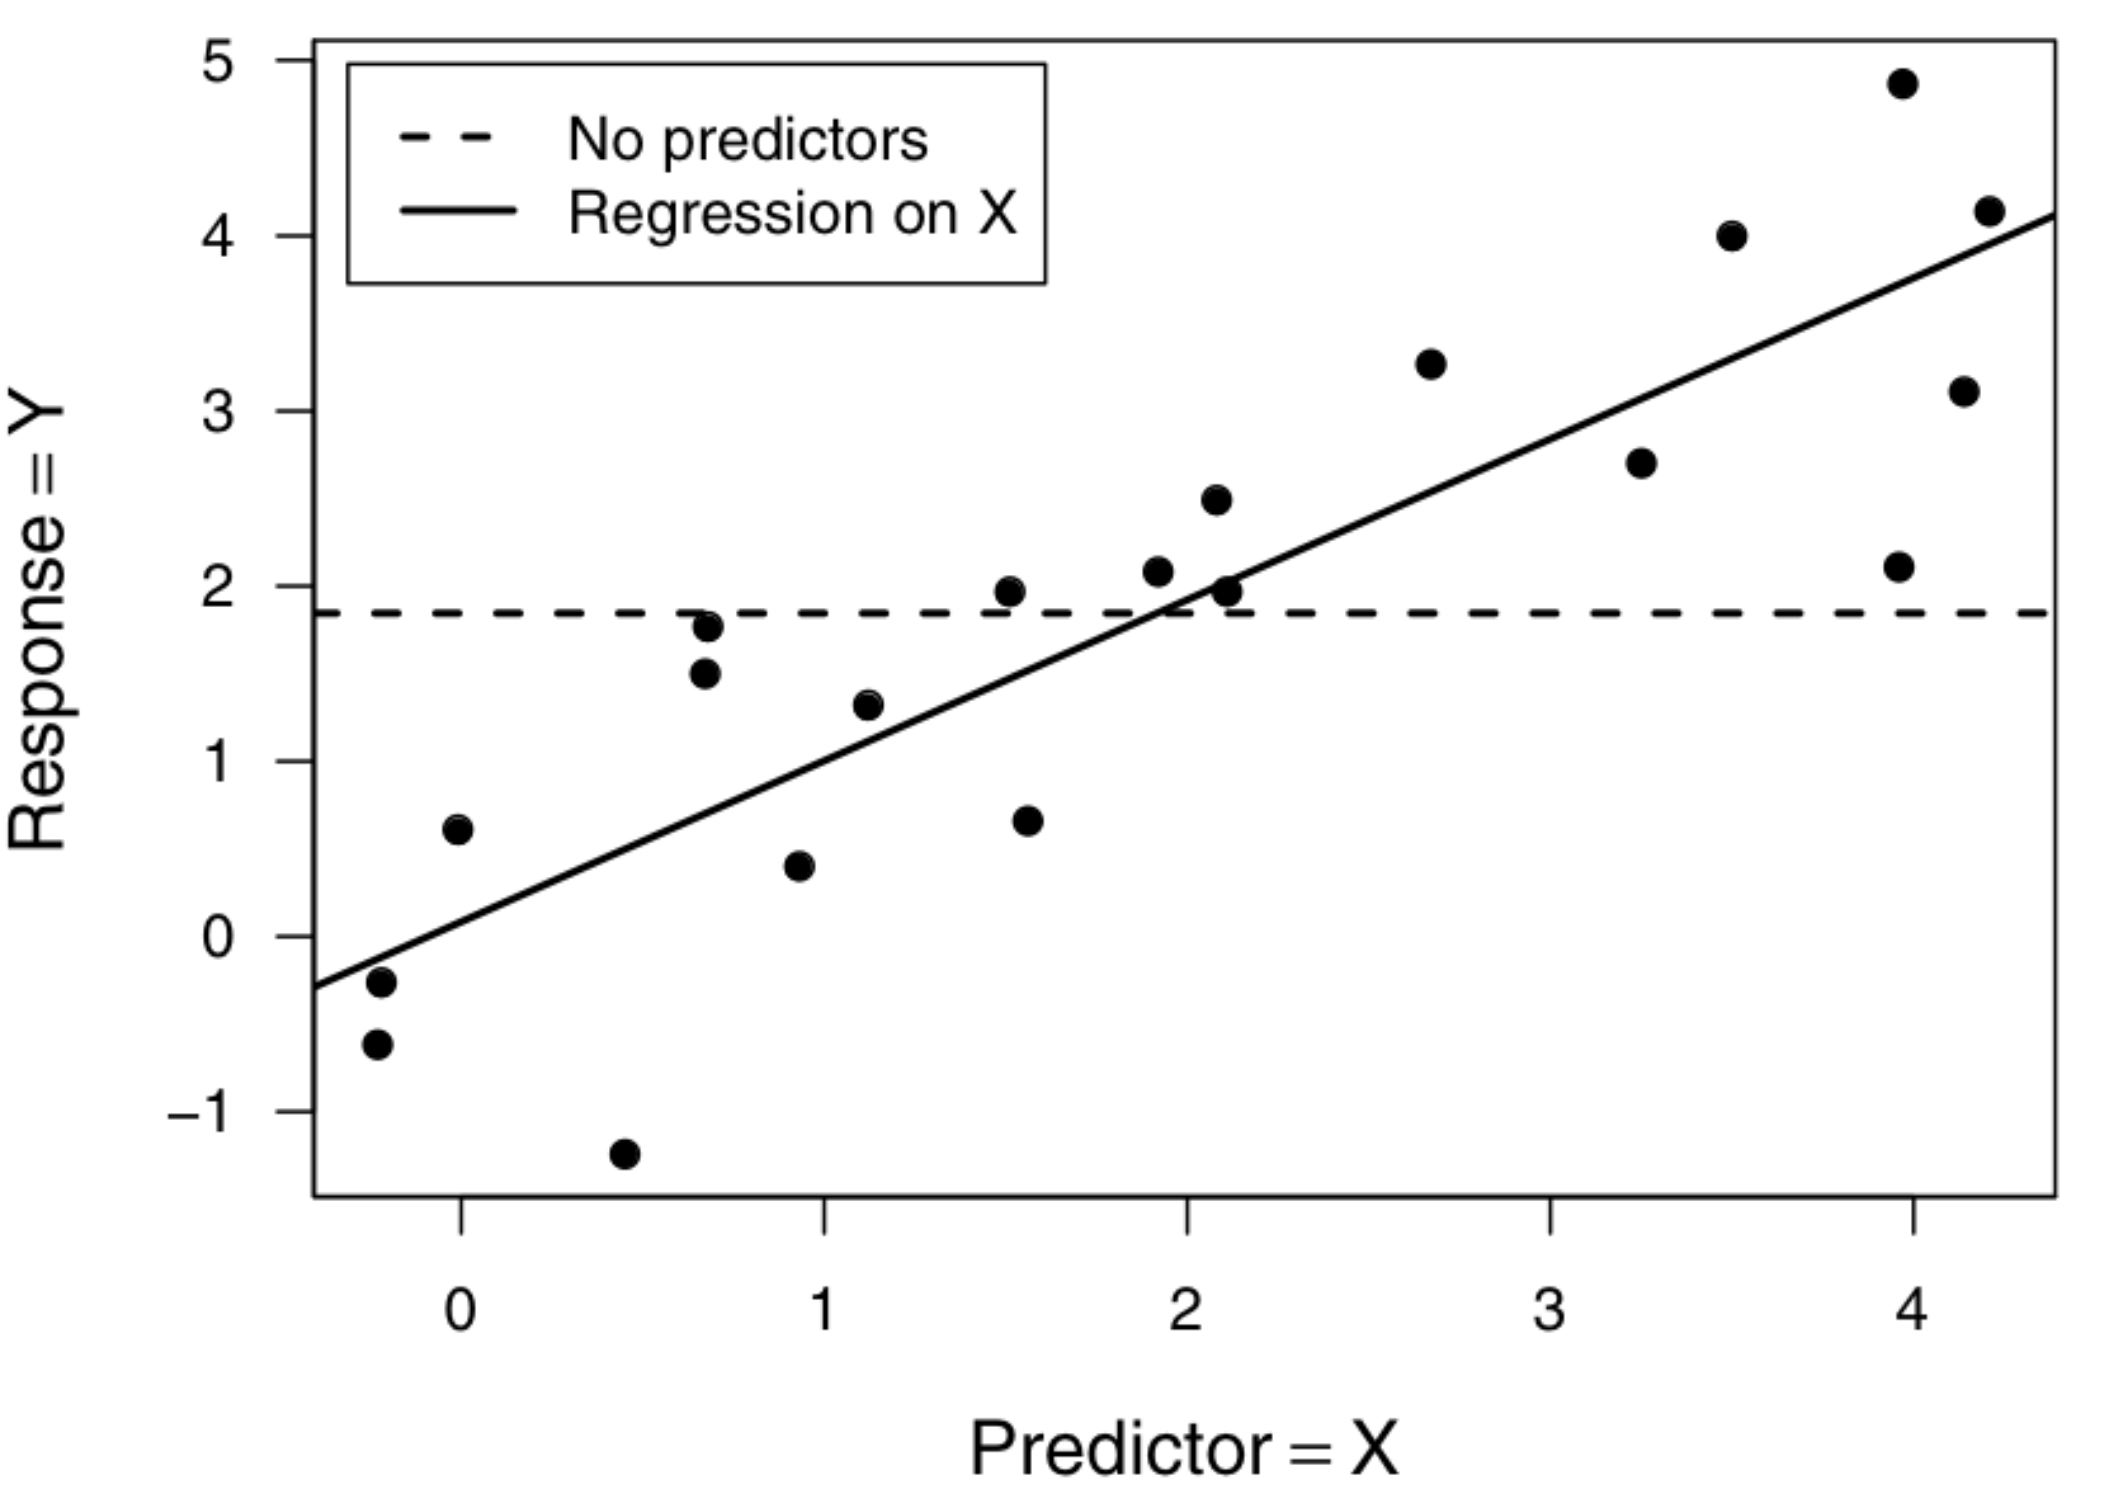
\includegraphics[width=1\textwidth]{fig9.png}
\end{figure}
\noindent
LHS is the proportion of observed variability in response explained by regression on the predictor.\\
RHS is $1 - $ remaining unexplained variability.\\
Then define:
\[
R^2 = \frac{SS_{\text{reg}}}{SYY} = 1 - \frac{RSS}{SYY}
\]
\[
\textcolor{red}{\quad R^2 :  \text{coefficient of determination}}
\]
\begin{itemize}
    \item Scale-free
    \item One-number summary of the strength of the relationship of $y$ on $x$.
\end{itemize}
\textbf{Fact: }
\[
R^2 = \frac{SS_{\text{reg}}}{SYY} = \frac{(SXY)^2}{SXX \cdot SYY} = r_{xy}^2
\]
\[
\textcolor{red}{\quad r_{xy}^2 \text{: square of sample correlation}}
\]

\subsection*{Adjusted $R^2$}
\[
R_{\text{adj}}^2 = 1 - \frac{RSS / df}{SYY / (n - 1)}
\]
 - Adds correction for degrees of freedom (df). 

 - Can facilitate comparing models in multiple linear regression.
\begin{figure}[H]
    \centering
    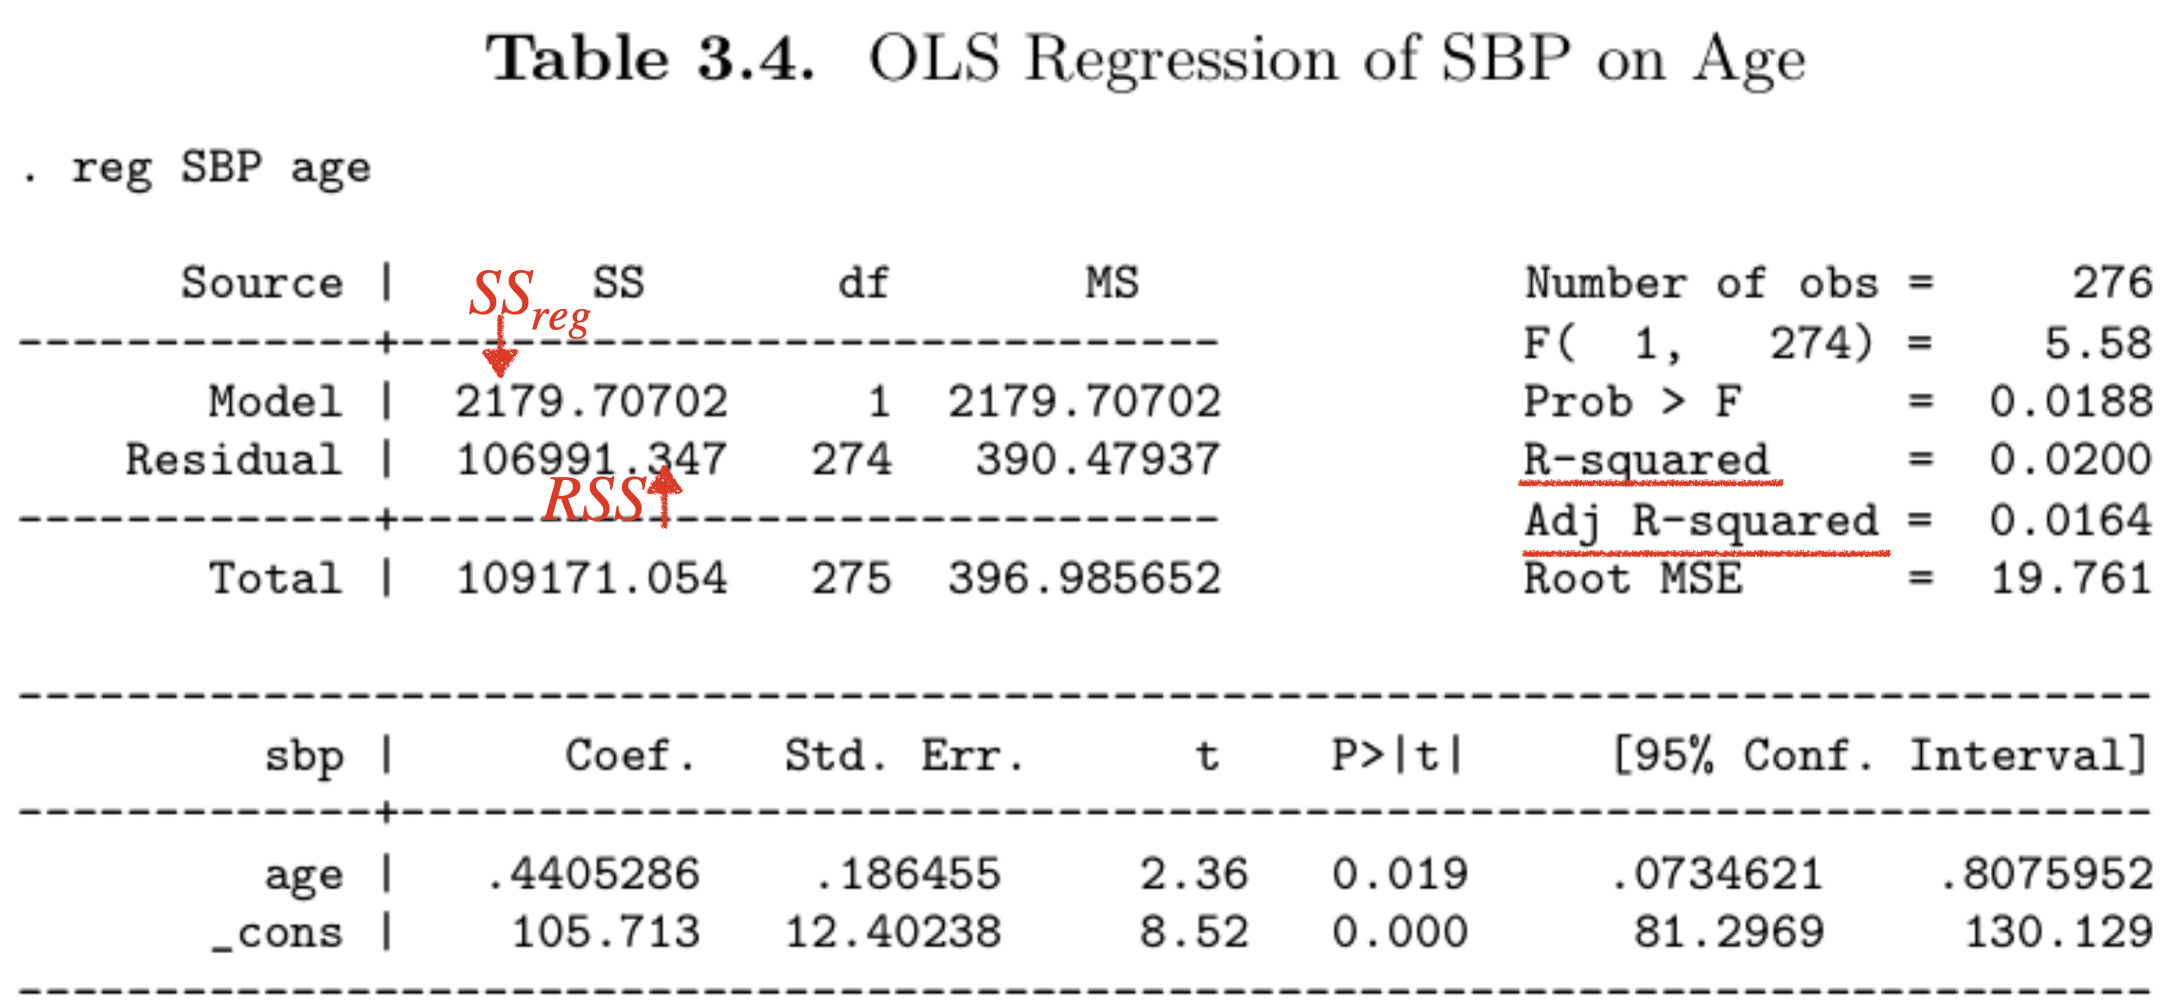
\includegraphics[width=1\textwidth]{fig10.png}
\end{figure}

\newpage

\subsection*{Residuals}
Recall: $\hat{e_i} = y_i - \hat{y_i}$\\
Residuals are used to find failures of assumptions.
\begin{figure}[H]
    \centering
    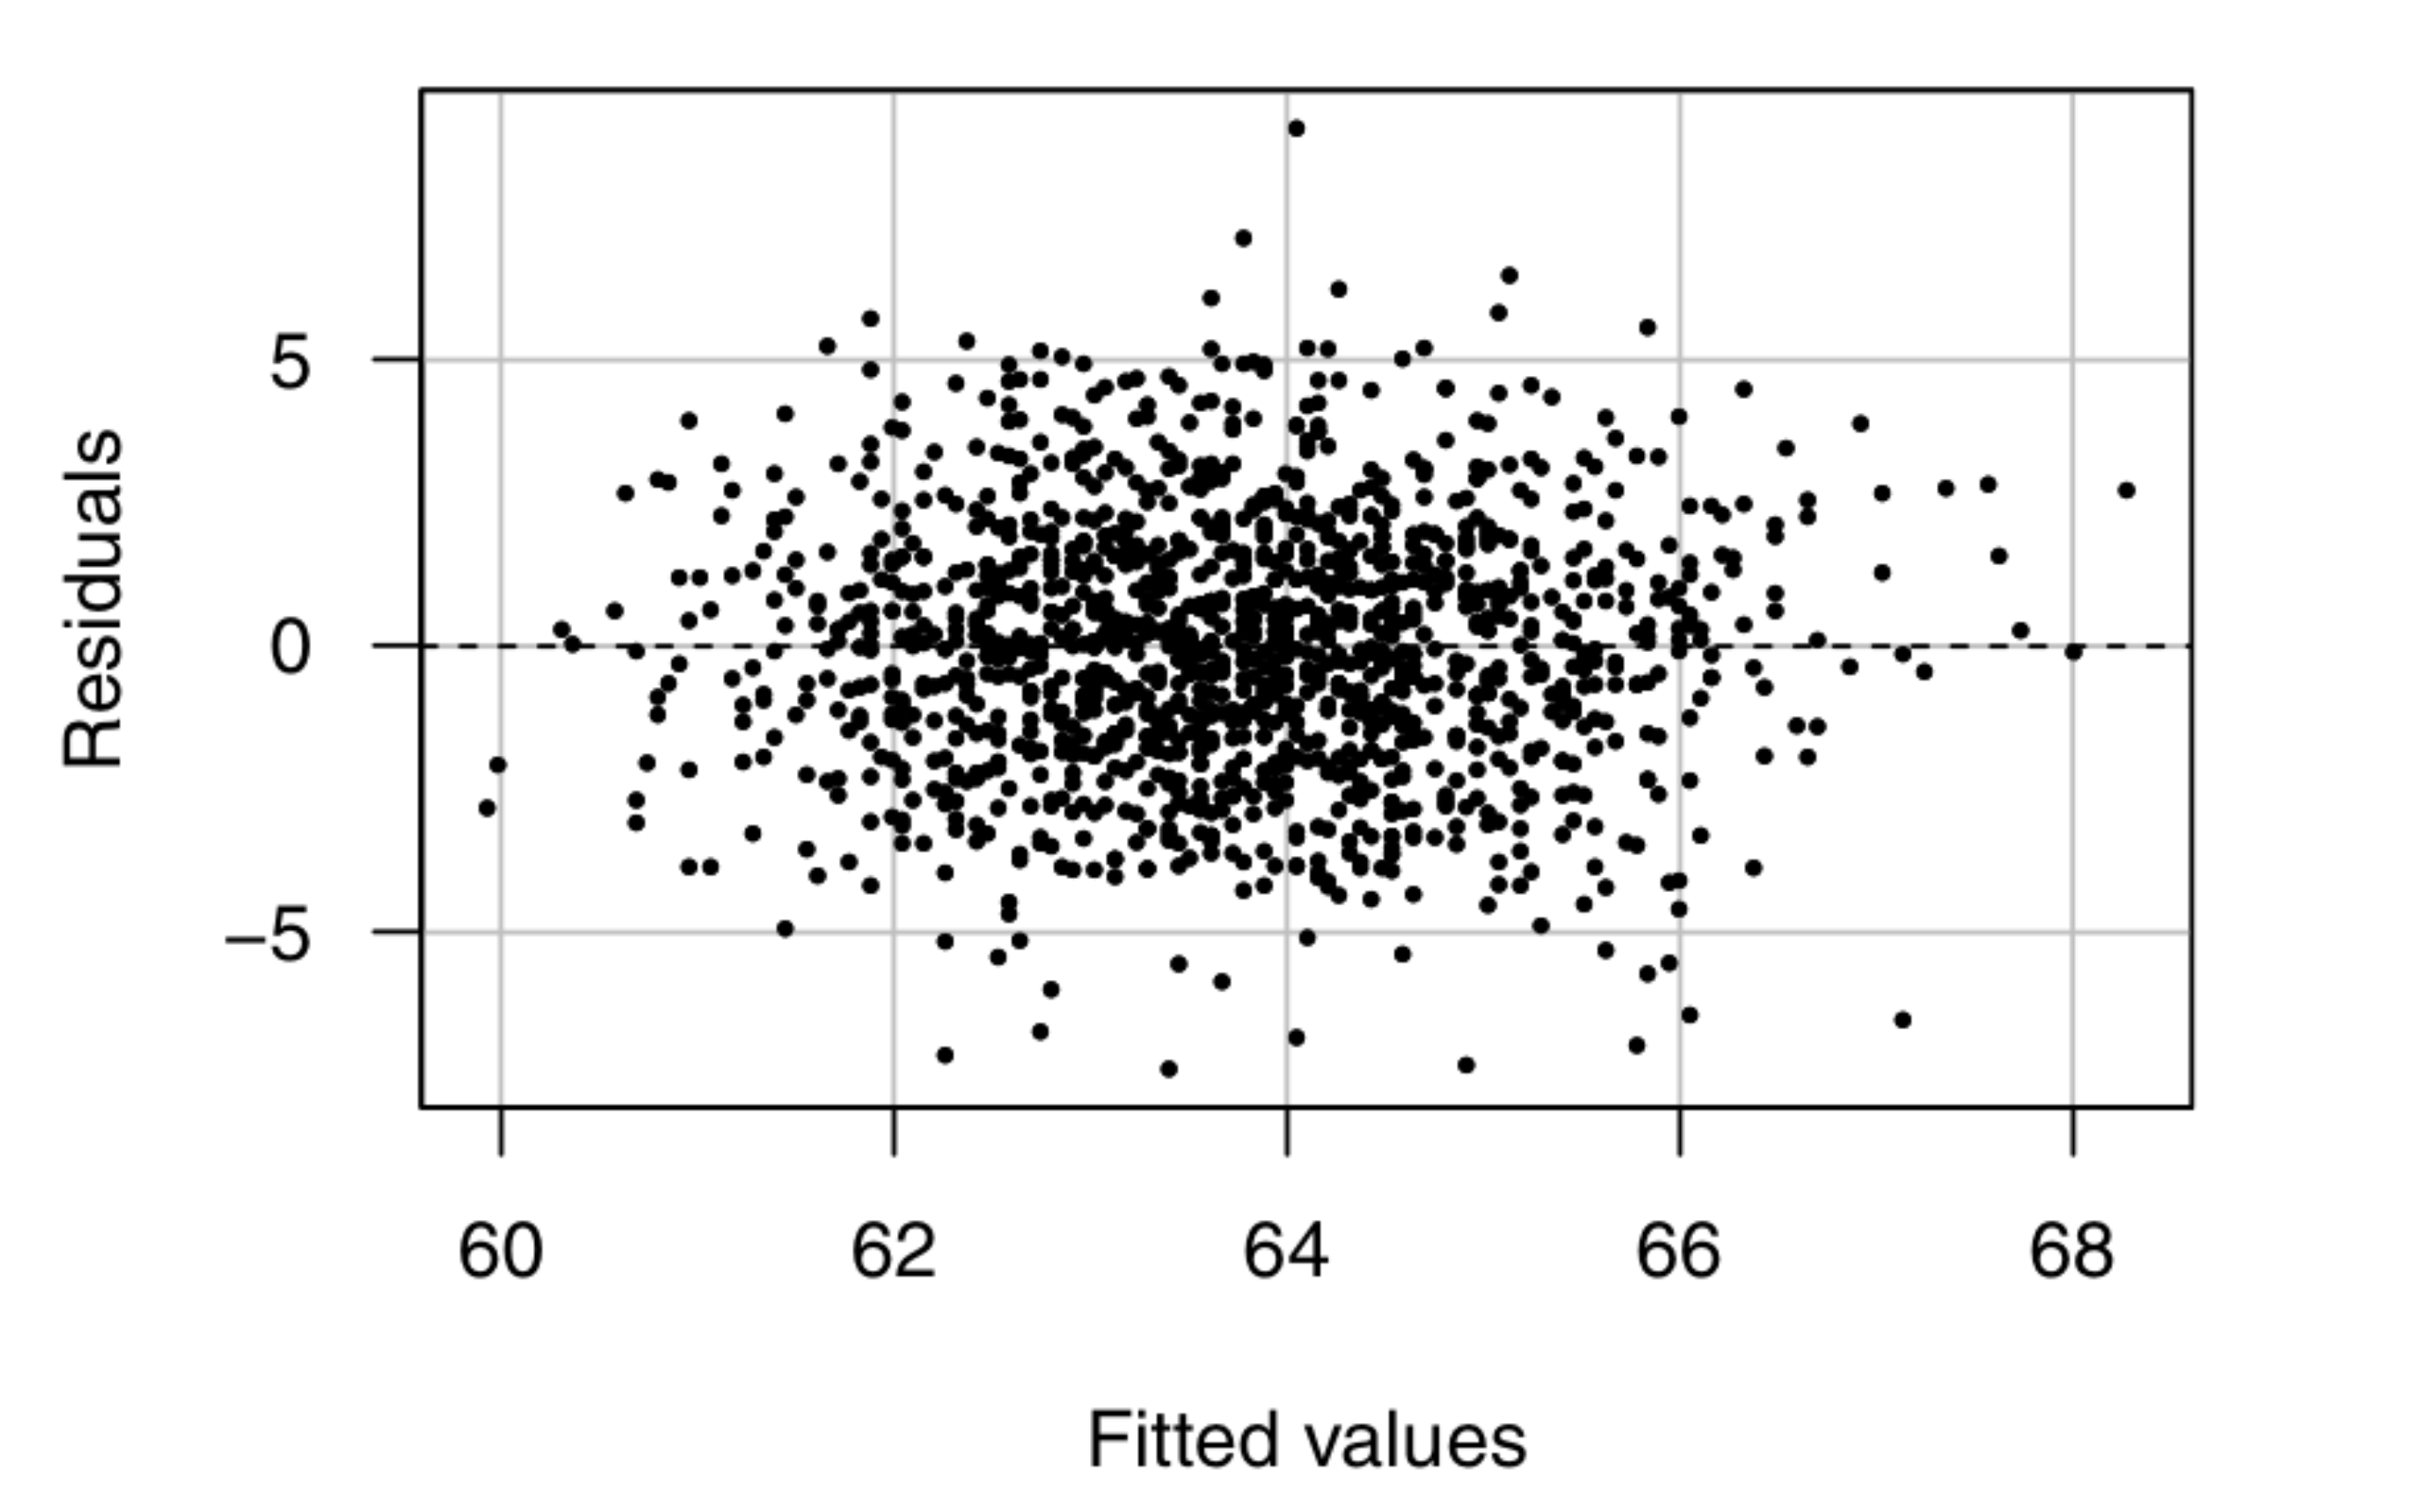
\includegraphics[width=1\textwidth]{fig11.png}
\end{figure}
\noindent
No pattern observed. \\
Residuals are small compared to fitted values. \\
\textcolor{red}{(Will say more on residual diagnostics later.)}

\end{document}






































\end{document}

